% Preamble
\documentclass[10pt,letterpaper]{article}
\usepackage[spanish]{babel}

% Packages
\selectlanguage{spanish}
\usepackage[utf8]{inputenc} % For spanish (and international) letters like acents.
\usepackage{hyperref} % To create hyperlinks within the document.
\usepackage{graphicx} % To include graphics (pictures, images)
%\usepackage{svg} % To include SVG graphics
%\usepackage{epstopdf} % To include graphics (EPS file format)
\usepackage{float} % For the use of the parameter "H" in command "\begin{figure}[H]" (i.e. exact position of image in text)
\usepackage{verbatim} % For long comments
\usepackage{tikz} % For include Dia diagrams in .tex format

% Document environment
\begin{document}

% Top matter
\title{Documentación del sistema de consulta para el Laboratorio Audiovisual de Investigación Social}
\author{Rodrigo Eduardo Colín Rivera}
\date{\today}
\maketitle

\setcounter{secnumdepth}{0} % Non-numbering sections
\setcounter{tocdepth}{0} % Non-numnbering table of contents
\graphicspath{{Diagramas/}} % Path of the folder containing the images

\begin{abstract}
El Laboratorio Audiovisual de Investigación Social (LAIS) del Instituto Mora consta de una colección archivística para materiales audiovisuales cuyos registros actuales se encuentran en formato de hojas de cálculo. Un mejor tratamiento de esta información requiere el uso de bases de datos y una interfaz (preferentemente web) para realizar la consulta e inserción de los registros e información que describen dichos materiales con el objetivo de facilitar las tareas de catalogación dentro y fuera del laboratorio.

Se mencionará la forma de catalogación actual, la propuesta del sistema, los problemas y soluciones que brinda el sistema, la elección de las tecnologías involucradas en la implementación, el alcance o usos del sistema, los prototipos y las propuestas a considerar para el futuro desarrollo.
\end{abstract}

\section{Antecedentes y problemática actual}
El Laboratorio Audiovisual de Investigación Social (LAIS) del Instituto Mora consta de una colección archivística para materiales audiovisuales cuyos registros actuales se encuentran en formato de hojas de cálculo a través del programa Microsoft Excel ingresando diversos rubros que integran la ficha de documentación de cada material audiovisual con base en la adaptación de la norma ISAD(G) (\textit{General International Standard Archival Description}), de la cual se mencionará a detalle más adelante.

La problemática principal con esta manera de catalogación es que resulta complicado buscar o filtrar los registros. Aunque este problema es la base de la propuesta del sistema, existen otros problemas relacionados tales como: La integridad de la información entre los libros de las hojas de cálculo, la cantidad de usuarios que pueden consultar estos registros y la manipulación de los datos.

\section{Propuesta para el sistema de consulta del LAIS}
La propuesta principal está apoyada en la idea de crear una base de datos para el manejo actual y futuro de las fichas de documentación de los materiales audiovisuales del LAIS.

\subsection{Diferencias entre hojas de cálculo y bases de datos}
Aunque ambas opciones tienen como objetivo almacenar conjuntos de datos, hay diferencias importantes a considerar y que se mencionan a continuación:

\begin{comment}
\begin{description}
	\item[Objetivo] \hfill \\
		Las hojas de cálculo se emplean principalmente para cálculos numéricos a través del uso de diversas fórmulas matemáticas. Las bases de datos tienen como objetivo almacenar datos en un servidor.
	\item[Almacenamiento] \hfill \\
		Las hojas de cálculo se almacenan en archivos conocidos como libros, cada uno de ellos tiene una o varias hojas de cálculo con filas y columnas para describir los datos. Las bases de datos contienen tablas, que a su vez contienen registros o renglones, donde cada valor le corresponde a una columna o tipo de dato.
	\item[Tecnologías] \hfill \\
		Los programas para uso de hojas de cálculo más comunes con Microsoft Excel, OppenOffice/LibreOffice Calc o Google Docs/Google Drive. Los manejadores de bases de datos comunes son 
\end{description}
\end{comment}

\begin{center}
	\begin{tabular}{| l | p{5cm} | p{5cm} |}
		\hline
		 & Hoja de cálculo & Base de datos \\ \hline
		 
		 Objetivo 
		 	& Realizar cálculos numéricos a través del uso de diversas fórmulas aritméticas. 
		 	& Almacenar datos en un servidor. \\
		 \hline
		 Almacenamiento
		 	& En archivos (libros) que contienen una o varias hojas de cálculo con filas y columnas para describir los datos.
		 	& En tablas que contienen registros (renglones) donde cada valor le corresponde un tipo de dato (columna)\\
		 \hline
		 Manejo
		 	& Cualquier persona con un conocimiento básico puede manipular, ordenar o filtrar datos.
		 	& Programador o persona encargada de la base de datos realiza consultas a través del lenguaje de programación SQL (\textit{Structured Query Language}). Requiere una interfaz de usuario para una fácil manipulación de la base. \\
		 \hline
		 Complejidad (datos)
		 	& Los datos son sencillos de manejar pero a mayor cantidad, mayor complejidad.
		 	& El modelo relacional permite mantener unidades organizadas para los datos (tablas) \\
		 	\hline
		 Repetición de datos
		 	& Se pueden presentar repetición o redundancia de datos.
		 	& Si el diseño de la base de datos es correcta, no se permite redundancia de información. \\
		 	\hline
		 Modificaciones
		 	& Una sola persona puede modificar a la vez. Varias personas con copia del original pueden hacer modificaciones pero al combinar la información queda sujeta a errores humanos.
		 	& Los manejadores (programas) de bases de datos permite multiusuarios y mecanismos de control en las modificaciones. \\
		 	\hline
		 Presentación
		 	& Adecuado para incrustar en documentos escritos o mostrar gráficas relativas a los datos contenidos.
		 	& Solamente a través de una interfaz de usuario se pueden presentar los datos. El formato varia según la implementación. \\
		 	\hline
	\end{tabular}
\end{center}

\section{Esquema general del sistema}
Debido a que no la manipulación de la base de datos requiere de instrucciones en el lenguaje de consulta SQL, para que los usuarios puedan realizar las operaciones comunes como consultar, buscar, insertar y borrar registros, se debe crear una interfaz que facilite estas tareas.

La figura~\ref{fig:esquema_general} muestra el diseño general separando la base de datos de la aplicación web. La aplicación web se comunica con la base de datos a partir de peticiones que devuelven los datos necesarios (en caso de consulta, búsqueda o inserción de datos) o la modificación correspondiente (en caso de modificar o eliminar datos).

También muestra que la base de datos está basada en las hojas de cálculo existentes, de esta manera no hay necesidad de reescribir toda la información, más bien es importada a la base de datos.

Finalmente se muestra las responsabilidades del programador para el diseño y creación de la base de datos y la interfaz web, mientras que los usuarios solamente requieren conocer el resultado de la interfaz web, es decir, una página en internet amigable y funcional para manipular la base de datos.

\begin{figure}[H]
	\centering
	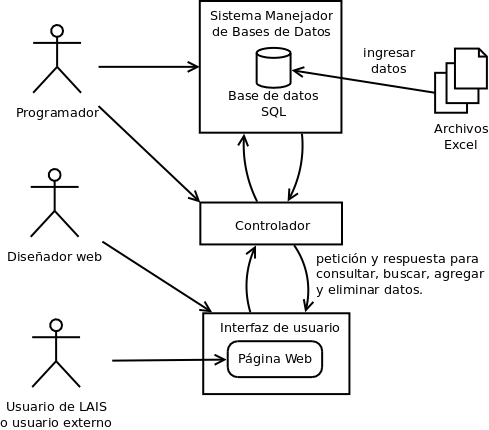
\includegraphics[width=0.8\textwidth]{EsquemaGeneral.png}
	\caption{Esquema general del sistema de consulta}
	\label{fig:esquema_general}
\end{figure}

\subsection{Casos de uso}
La figura~\ref{fig:caso_de_uso} muestra el diagrama de casos de uso que representa a los usuarios y las acciones principales del sistema.
\begin{figure}[H]
	\centering
	%% Graphic for TeX using PGF
% Title: /home/rodrigo/Instituto Mora/SistemaConsultaLAIS/Documentacion/CasosDeUso.dia
% Creator: Dia v0.97.2
% CreationDate: Thu Mar 12 11:48:33 2015
% For: rodrigo
% \usepackage{tikz}
% The following commands are not supported in PSTricks at present
% We define them conditionally, so when they are implemented,
% this pgf file will use them.
\ifx\du\undefined
  \newlength{\du}
\fi
\setlength{\du}{15\unitlength}
\begin{tikzpicture}
\pgftransformxscale{1.000000}
\pgftransformyscale{-1.000000}
\definecolor{dialinecolor}{rgb}{0.000000, 0.000000, 0.000000}
\pgfsetstrokecolor{dialinecolor}
\definecolor{dialinecolor}{rgb}{1.000000, 1.000000, 1.000000}
\pgfsetfillcolor{dialinecolor}
\pgfsetlinewidth{0.100000\du}
\pgfsetdash{}{0pt}
\pgfsetdash{}{0pt}
\pgfsetmiterjoin
\definecolor{dialinecolor}{rgb}{0.749020, 0.749020, 0.749020}
\pgfsetstrokecolor{dialinecolor}
\draw (16.757500\du,2.750000\du)--(16.757500\du,20.400000\du)--(29.757500\du,20.400000\du)--(29.757500\du,2.750000\du)--cycle;
\pgfsetlinewidth{0.100000\du}
\pgfsetdash{}{0pt}
\definecolor{dialinecolor}{rgb}{1.000000, 1.000000, 1.000000}
\pgfsetfillcolor{dialinecolor}
\pgfpathellipse{\pgfpoint{9.884375\du}{12.900000\du}}{\pgfpoint{0.300000\du}{0\du}}{\pgfpoint{0\du}{0.300000\du}}
\pgfusepath{fill}
\definecolor{dialinecolor}{rgb}{0.000000, 0.000000, 0.000000}
\pgfsetstrokecolor{dialinecolor}
\pgfpathellipse{\pgfpoint{9.884375\du}{12.900000\du}}{\pgfpoint{0.300000\du}{0\du}}{\pgfpoint{0\du}{0.300000\du}}
\pgfusepath{stroke}
\definecolor{dialinecolor}{rgb}{0.000000, 0.000000, 0.000000}
\pgfsetstrokecolor{dialinecolor}
\draw (8.684375\du,13.500000\du)--(11.084375\du,13.500000\du);
\definecolor{dialinecolor}{rgb}{0.000000, 0.000000, 0.000000}
\pgfsetstrokecolor{dialinecolor}
\draw (9.884375\du,13.200000\du)--(9.884375\du,14.700000\du);
\definecolor{dialinecolor}{rgb}{0.000000, 0.000000, 0.000000}
\pgfsetstrokecolor{dialinecolor}
\draw (9.884375\du,14.700000\du)--(8.684375\du,16.000000\du);
\definecolor{dialinecolor}{rgb}{0.000000, 0.000000, 0.000000}
\pgfsetstrokecolor{dialinecolor}
\draw (9.884375\du,14.700000\du)--(11.084375\du,16.000000\du);
% setfont left to latex
\definecolor{dialinecolor}{rgb}{0.000000, 0.000000, 0.000000}
\pgfsetstrokecolor{dialinecolor}
\node at (9.884375\du,17.195000\du){Usuario interno };
% setfont left to latex
\definecolor{dialinecolor}{rgb}{0.000000, 0.000000, 0.000000}
\pgfsetstrokecolor{dialinecolor}
\node at (9.884375\du,17.995000\du){del LAIS};
\pgfsetlinewidth{0.100000\du}
\pgfsetdash{}{0pt}
{\pgfsetcornersarced{\pgfpoint{1.000000\du}{1.000000\du}}\definecolor{dialinecolor}{rgb}{1.000000, 1.000000, 1.000000}
\pgfsetfillcolor{dialinecolor}
\fill (19.235625\du,3.937500\du)--(19.235625\du,6.537500\du)--(27.753125\du,6.537500\du)--(27.753125\du,3.937500\du)--cycle;
}{\pgfsetcornersarced{\pgfpoint{1.000000\du}{1.000000\du}}\definecolor{dialinecolor}{rgb}{0.000000, 0.000000, 0.000000}
\pgfsetstrokecolor{dialinecolor}
\draw (19.235625\du,3.937500\du)--(19.235625\du,6.537500\du)--(27.753125\du,6.537500\du)--(27.753125\du,3.937500\du)--cycle;
}% setfont left to latex
\definecolor{dialinecolor}{rgb}{0.000000, 0.000000, 0.000000}
\pgfsetstrokecolor{dialinecolor}
\node at (23.494375\du,5.032500\du){Consultar registro};
% setfont left to latex
\definecolor{dialinecolor}{rgb}{0.000000, 0.000000, 0.000000}
\pgfsetstrokecolor{dialinecolor}
\node at (23.494375\du,5.832500\du){de material audiovisual};
\pgfsetlinewidth{0.100000\du}
\pgfsetdash{}{0pt}
{\pgfsetcornersarced{\pgfpoint{1.000000\du}{1.000000\du}}\definecolor{dialinecolor}{rgb}{1.000000, 1.000000, 1.000000}
\pgfsetfillcolor{dialinecolor}
\fill (19.235625\du,12.237500\du)--(19.235625\du,14.837500\du)--(27.753125\du,14.837500\du)--(27.753125\du,12.237500\du)--cycle;
}{\pgfsetcornersarced{\pgfpoint{1.000000\du}{1.000000\du}}\definecolor{dialinecolor}{rgb}{0.000000, 0.000000, 0.000000}
\pgfsetstrokecolor{dialinecolor}
\draw (19.235625\du,12.237500\du)--(19.235625\du,14.837500\du)--(27.753125\du,14.837500\du)--(27.753125\du,12.237500\du)--cycle;
}% setfont left to latex
\definecolor{dialinecolor}{rgb}{0.000000, 0.000000, 0.000000}
\pgfsetstrokecolor{dialinecolor}
\node at (23.494375\du,13.332500\du){Agregar nuevo registro};
% setfont left to latex
\definecolor{dialinecolor}{rgb}{0.000000, 0.000000, 0.000000}
\pgfsetstrokecolor{dialinecolor}
\node at (23.494375\du,14.132500\du){de material audiovisual};
\pgfsetlinewidth{0.100000\du}
\pgfsetdash{}{0pt}
{\pgfsetcornersarced{\pgfpoint{1.000000\du}{1.000000\du}}\definecolor{dialinecolor}{rgb}{1.000000, 1.000000, 1.000000}
\pgfsetfillcolor{dialinecolor}
\fill (18.611875\du,16.387500\du)--(18.611875\du,18.987500\du)--(28.376875\du,18.987500\du)--(28.376875\du,16.387500\du)--cycle;
}{\pgfsetcornersarced{\pgfpoint{1.000000\du}{1.000000\du}}\definecolor{dialinecolor}{rgb}{0.000000, 0.000000, 0.000000}
\pgfsetstrokecolor{dialinecolor}
\draw (18.611875\du,16.387500\du)--(18.611875\du,18.987500\du)--(28.376875\du,18.987500\du)--(28.376875\du,16.387500\du)--cycle;
}% setfont left to latex
\definecolor{dialinecolor}{rgb}{0.000000, 0.000000, 0.000000}
\pgfsetstrokecolor{dialinecolor}
\node at (23.494375\du,17.482500\du){Modificar registro existente};
% setfont left to latex
\definecolor{dialinecolor}{rgb}{0.000000, 0.000000, 0.000000}
\pgfsetstrokecolor{dialinecolor}
\node at (23.494375\du,18.282500\du){de material audiovisual};
\pgfsetlinewidth{0.100000\du}
\pgfsetdash{}{0pt}
{\pgfsetcornersarced{\pgfpoint{1.000000\du}{1.000000\du}}\definecolor{dialinecolor}{rgb}{1.000000, 1.000000, 1.000000}
\pgfsetfillcolor{dialinecolor}
\fill (19.235625\du,8.187500\du)--(19.235625\du,10.787500\du)--(27.753125\du,10.787500\du)--(27.753125\du,8.187500\du)--cycle;
}{\pgfsetcornersarced{\pgfpoint{1.000000\du}{1.000000\du}}\definecolor{dialinecolor}{rgb}{0.000000, 0.000000, 0.000000}
\pgfsetstrokecolor{dialinecolor}
\draw (19.235625\du,8.187500\du)--(19.235625\du,10.787500\du)--(27.753125\du,10.787500\du)--(27.753125\du,8.187500\du)--cycle;
}% setfont left to latex
\definecolor{dialinecolor}{rgb}{0.000000, 0.000000, 0.000000}
\pgfsetstrokecolor{dialinecolor}
\node at (23.494375\du,9.282500\du){Realizar búsquedas};
% setfont left to latex
\definecolor{dialinecolor}{rgb}{0.000000, 0.000000, 0.000000}
\pgfsetstrokecolor{dialinecolor}
\node at (23.494375\du,10.082500\du){de material audiovisual};
\pgfsetlinewidth{0.100000\du}
\pgfsetdash{}{0pt}
\pgfsetdash{}{0pt}
\pgfsetbuttcap
{
\definecolor{dialinecolor}{rgb}{0.000000, 0.000000, 0.000000}
\pgfsetfillcolor{dialinecolor}
% was here!!!
\definecolor{dialinecolor}{rgb}{0.000000, 0.000000, 0.000000}
\pgfsetstrokecolor{dialinecolor}
\draw (12.404829\du,12.149561\du)--(19.235625\du,5.237500\du);
}
\pgfsetlinewidth{0.100000\du}
\pgfsetdash{}{0pt}
\pgfsetdash{}{0pt}
\pgfsetbuttcap
{
\definecolor{dialinecolor}{rgb}{0.000000, 0.000000, 0.000000}
\pgfsetfillcolor{dialinecolor}
% was here!!!
\definecolor{dialinecolor}{rgb}{0.000000, 0.000000, 0.000000}
\pgfsetstrokecolor{dialinecolor}
\draw (12.404829\du,14.386670\du)--(19.235625\du,13.537500\du);
}
\pgfsetlinewidth{0.100000\du}
\pgfsetdash{}{0pt}
\pgfsetdash{}{0pt}
\pgfsetbuttcap
{
\definecolor{dialinecolor}{rgb}{0.000000, 0.000000, 0.000000}
\pgfsetfillcolor{dialinecolor}
% was here!!!
\definecolor{dialinecolor}{rgb}{0.000000, 0.000000, 0.000000}
\pgfsetstrokecolor{dialinecolor}
\draw (12.424214\du,15.569409\du)--(18.611875\du,17.687500\du);
}
\pgfsetlinewidth{0.100000\du}
\pgfsetdash{}{0pt}
\pgfsetdash{}{0pt}
\pgfsetbuttcap
{
\definecolor{dialinecolor}{rgb}{0.000000, 0.000000, 0.000000}
\pgfsetfillcolor{dialinecolor}
% was here!!!
\definecolor{dialinecolor}{rgb}{0.000000, 0.000000, 0.000000}
\pgfsetstrokecolor{dialinecolor}
\draw (12.404829\du,13.295068\du)--(19.235625\du,9.487500\du);
}
% setfont left to latex
\definecolor{dialinecolor}{rgb}{0.000000, 0.000000, 0.000000}
\pgfsetstrokecolor{dialinecolor}
\node[anchor=west] at (20.307500\du,2.150000\du){Sistema de consulta};
\pgfsetlinewidth{0.100000\du}
\pgfsetdash{}{0pt}
\definecolor{dialinecolor}{rgb}{1.000000, 1.000000, 1.000000}
\pgfsetfillcolor{dialinecolor}
\pgfpathellipse{\pgfpoint{9.884375\du}{4.117500\du}}{\pgfpoint{0.300000\du}{0\du}}{\pgfpoint{0\du}{0.300000\du}}
\pgfusepath{fill}
\definecolor{dialinecolor}{rgb}{0.000000, 0.000000, 0.000000}
\pgfsetstrokecolor{dialinecolor}
\pgfpathellipse{\pgfpoint{9.884375\du}{4.117500\du}}{\pgfpoint{0.300000\du}{0\du}}{\pgfpoint{0\du}{0.300000\du}}
\pgfusepath{stroke}
\definecolor{dialinecolor}{rgb}{0.000000, 0.000000, 0.000000}
\pgfsetstrokecolor{dialinecolor}
\draw (8.684375\du,4.717500\du)--(11.084375\du,4.717500\du);
\definecolor{dialinecolor}{rgb}{0.000000, 0.000000, 0.000000}
\pgfsetstrokecolor{dialinecolor}
\draw (9.884375\du,4.417500\du)--(9.884375\du,5.917500\du);
\definecolor{dialinecolor}{rgb}{0.000000, 0.000000, 0.000000}
\pgfsetstrokecolor{dialinecolor}
\draw (9.884375\du,5.917500\du)--(8.684375\du,7.217500\du);
\definecolor{dialinecolor}{rgb}{0.000000, 0.000000, 0.000000}
\pgfsetstrokecolor{dialinecolor}
\draw (9.884375\du,5.917500\du)--(11.084375\du,7.217500\du);
% setfont left to latex
\definecolor{dialinecolor}{rgb}{0.000000, 0.000000, 0.000000}
\pgfsetstrokecolor{dialinecolor}
\node at (9.884375\du,8.412500\du){Usuario externo };
% setfont left to latex
\definecolor{dialinecolor}{rgb}{0.000000, 0.000000, 0.000000}
\pgfsetstrokecolor{dialinecolor}
\node at (9.884375\du,9.212500\du){del LAIS};
\pgfsetlinewidth{0.100000\du}
\pgfsetdash{}{0pt}
\pgfsetdash{}{0pt}
\pgfsetbuttcap
{
\definecolor{dialinecolor}{rgb}{0.000000, 0.000000, 0.000000}
\pgfsetfillcolor{dialinecolor}
% was here!!!
\definecolor{dialinecolor}{rgb}{0.000000, 0.000000, 0.000000}
\pgfsetstrokecolor{dialinecolor}
\draw (12.523546\du,5.725586\du)--(19.235625\du,5.237500\du);
}
\pgfsetlinewidth{0.100000\du}
\pgfsetdash{}{0pt}
\pgfsetdash{}{0pt}
\pgfsetbuttcap
{
\definecolor{dialinecolor}{rgb}{0.000000, 0.000000, 0.000000}
\pgfsetfillcolor{dialinecolor}
% was here!!!
\definecolor{dialinecolor}{rgb}{0.000000, 0.000000, 0.000000}
\pgfsetstrokecolor{dialinecolor}
\draw (19.235625\du,9.487500\du)--(12.523546\du,6.925049\du);
}
\end{tikzpicture}

	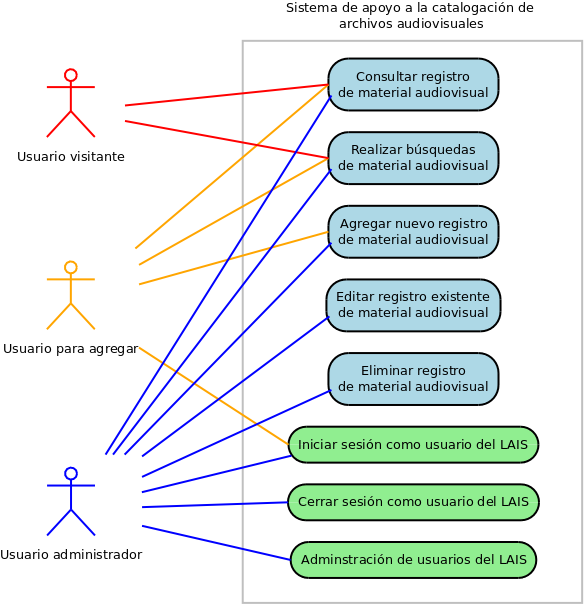
\includegraphics[width=0.8\textwidth]{CasosDeUso.png}
	\caption{Diagrama de casos de uso}
	\label{fig:caso_de_uso}
\end{figure}

\section{Selección de tecnologías}
Existen diversas maneras de implementar el sistema y la selección de las tecnologías necesarias para su implementación es importante para que cumplan con los requisitos y se adapte adecuadamente a las necesidades del LAIS.
\subsection{MySQL}
MySQL es el Sistema Manejador de Bases de Datos Relacionales de código abierto (open source) más ampliamente utilizado y que actualmente es respaldada para su desarrollo por la corporación Oracle.
MySQL es una elección común para uso de bases de datos para aplicaciones web, pues es un componente del conjunto de software denomidado LAMP (acrónimo de "Linux, Apache, MySQL, Perl/PHP/Python"). Debido a que en el LAIS se cuenta con un servidor Apache en Linux, es conveniente que la elección para el manejo de la base de datos sea con MySQL.

\subsection{MySQL Workbench}
Este entorno de desarrollo integrado (IDE por sus siglas en inglés) permite el diseño, desarrollo y administración de manera visual de la base de datos. Especialmente útil para programadores ya que está disponible para todos los sistemas operativos (Linux, Mac y Windows) y solo requiere hacer la conexión con el servidor para poder administrarla de manera remota.

\subsection{PHP}
Debido a que se requiere de una interfaz web para hacer uso de la base de datos, dicha interfaz requiere un lenguaje de programación que permita hacer desarrollo web del lado del servidor. PHP es un lenguaje ampliamente usado y probado.

En particular, el uso del complemento PDO (PHP Database Object) permite realizar operaciones comunes de la base de datos (como conectarse, agregar registros y realizar consultas) desde una página web utilizando la filosofía de la orientación a objetos, lo cual también facilita la programación de la interfaz o página web.

\subsection{HTML5 y Bootstrap}
Así como PHP es el intermediario con la base de datos, el intermediario que hace uso de esta tecnología y la pone a disposición del usuario es HTML. HTML es un lenguaje de marcado para crear páginas web que facilitan el uso de la base de datos desde un ambiente más amigable. El estándar actual recomendado se conoce como HTML5 y es el estándar con el que se desarrollará.

Bootstrap es un conjunto de herramientas para la creación de páginas web y aplicaciones web, principalmente usado para darle estilo a componentes como la tipografía, formularios, botónes y otros componentes de la interfaz. Además permite diseño responsivo para que la interfaz web sea adecuada tanto en monitores grandes de computadoras de escritorio como para pantallas pequeñas de dispositivos móviles (smartphones y tablets).

\section{Diseño de la base de datos}
Las tablas y los campos o columnas que lo conforman están basadas en la descripción archivística existente en hojas de cálculo que hasta el momento han sido el modelo a seguir para la catalogación archivística.

\begin{figure}[H]
	\centering
	%% Graphic for TeX using PGF
% Title: /home/rodrigo/Instituto Mora/SistemaConsultaLAIS/Documentacion/Diagramas/EntidadRelacion.dia
% Creator: Dia v0.97.2
% CreationDate: Thu Mar 19 15:57:56 2015
% For: rodrigo
% \usepackage{tikz}
% The following commands are not supported in PSTricks at present
% We define them conditionally, so when they are implemented,
% this pgf file will use them.
\ifx\du\undefined
  \newlength{\du}
\fi
\setlength{\du}{15\unitlength}
\begin{tikzpicture}[scale=0.5]
\pgftransformxscale{1.000000}
\pgftransformyscale{-1.000000}
\definecolor{dialinecolor}{rgb}{0.000000, 0.000000, 0.000000}
\pgfsetstrokecolor{dialinecolor}
\definecolor{dialinecolor}{rgb}{1.000000, 1.000000, 1.000000}
\pgfsetfillcolor{dialinecolor}
\pgfsetlinewidth{0.100000\du}
\pgfsetdash{}{0pt}
\definecolor{dialinecolor}{rgb}{1.000000, 1.000000, 1.000000}
\pgfsetfillcolor{dialinecolor}
\fill (4.889590\du,14.211500\du)--(4.889590\du,15.111500\du)--(18.509590\du,15.111500\du)--(18.509590\du,14.211500\du)--cycle;
\definecolor{dialinecolor}{rgb}{0.000000, 0.000000, 0.000000}
\pgfsetstrokecolor{dialinecolor}
\draw (4.889590\du,14.211500\du)--(4.889590\du,15.111500\du)--(18.509590\du,15.111500\du)--(18.509590\du,14.211500\du)--cycle;
% setfont left to latex
\definecolor{dialinecolor}{rgb}{0.000000, 0.000000, 0.000000}
\pgfsetstrokecolor{dialinecolor}
\node at (11.699590\du,14.911500\du){area\_de\_identificacion};
\definecolor{dialinecolor}{rgb}{1.000000, 1.000000, 1.000000}
\pgfsetfillcolor{dialinecolor}
\fill (4.889590\du,15.111500\du)--(4.889590\du,36.111500\du)--(18.509590\du,36.111500\du)--(18.509590\du,15.111500\du)--cycle;
\definecolor{dialinecolor}{rgb}{0.000000, 0.000000, 0.000000}
\pgfsetstrokecolor{dialinecolor}
\draw (4.889590\du,15.111500\du)--(4.889590\du,36.111500\du)--(18.509590\du,36.111500\du)--(18.509590\du,15.111500\du)--cycle;
% setfont left to latex
\pgfsetlinewidth{0.010000\du}
\pgfsetmiterjoin
\definecolor{dialinecolor}{rgb}{0.000000, 0.000000, 0.000000}
\pgfsetfillcolor{dialinecolor}
\fill (5.039590\du,15.611500\du)--(5.139590\du,15.761500\du)--(5.239590\du,15.611500\du)--(5.139590\du,15.461500\du)--cycle;
\definecolor{dialinecolor}{rgb}{0.000000, 0.000000, 0.000000}
\pgfsetstrokecolor{dialinecolor}
\node[anchor=west] at (5.339590\du,15.911500\du){codigo\_de\_referencia};
\definecolor{dialinecolor}{rgb}{0.000000, 0.000000, 0.000000}
\pgfsetstrokecolor{dialinecolor}
\node[anchor=west] at (13.539590\du,15.911500\du){varchar(20)};
% setfont left to latex
\pgfsetlinewidth{0.010000\du}
\definecolor{dialinecolor}{rgb}{0.000000, 0.000000, 0.000000}
\pgfsetstrokecolor{dialinecolor}
\pgfpathellipse{\pgfpoint{5.139590\du}{16.411500\du}}{\pgfpoint{0.100000\du}{0\du}}{\pgfpoint{0\du}{0.100000\du}}
\pgfusepath{stroke}
\definecolor{dialinecolor}{rgb}{0.000000, 0.000000, 0.000000}
\pgfsetstrokecolor{dialinecolor}
\node[anchor=west] at (5.339590\du,16.711500\du){titulo\_propio};
\definecolor{dialinecolor}{rgb}{0.000000, 0.000000, 0.000000}
\pgfsetstrokecolor{dialinecolor}
\node[anchor=west] at (13.539590\du,16.711500\du){varchar(70)};
% setfont left to latex
\pgfsetlinewidth{0.010000\du}
\definecolor{dialinecolor}{rgb}{0.000000, 0.000000, 0.000000}
\pgfsetstrokecolor{dialinecolor}
\pgfpathellipse{\pgfpoint{5.139590\du}{17.211500\du}}{\pgfpoint{0.100000\du}{0\du}}{\pgfpoint{0\du}{0.100000\du}}
\pgfusepath{stroke}
\definecolor{dialinecolor}{rgb}{0.000000, 0.000000, 0.000000}
\pgfsetstrokecolor{dialinecolor}
\node[anchor=west] at (5.339590\du,17.511500\du){titulo\_paralelo};
\definecolor{dialinecolor}{rgb}{0.000000, 0.000000, 0.000000}
\pgfsetstrokecolor{dialinecolor}
\node[anchor=west] at (13.539590\du,17.511500\du){varchar(70)};
% setfont left to latex
\pgfsetlinewidth{0.010000\du}
\definecolor{dialinecolor}{rgb}{0.000000, 0.000000, 0.000000}
\pgfsetstrokecolor{dialinecolor}
\pgfpathellipse{\pgfpoint{5.139590\du}{18.011500\du}}{\pgfpoint{0.100000\du}{0\du}}{\pgfpoint{0\du}{0.100000\du}}
\pgfusepath{stroke}
\definecolor{dialinecolor}{rgb}{0.000000, 0.000000, 0.000000}
\pgfsetstrokecolor{dialinecolor}
\node[anchor=west] at (5.339590\du,18.311500\du){titulo\_atribuido};
\definecolor{dialinecolor}{rgb}{0.000000, 0.000000, 0.000000}
\pgfsetstrokecolor{dialinecolor}
\node[anchor=west] at (13.539590\du,18.311500\du){varchar(70)};
% setfont left to latex
\pgfsetlinewidth{0.010000\du}
\definecolor{dialinecolor}{rgb}{0.000000, 0.000000, 0.000000}
\pgfsetstrokecolor{dialinecolor}
\pgfpathellipse{\pgfpoint{5.139590\du}{18.811500\du}}{\pgfpoint{0.100000\du}{0\du}}{\pgfpoint{0\du}{0.100000\du}}
\pgfusepath{stroke}
\definecolor{dialinecolor}{rgb}{0.000000, 0.000000, 0.000000}
\pgfsetstrokecolor{dialinecolor}
\node[anchor=west] at (5.339590\du,19.111500\du){titulo\_de\_serie};
\definecolor{dialinecolor}{rgb}{0.000000, 0.000000, 0.000000}
\pgfsetstrokecolor{dialinecolor}
\node[anchor=west] at (13.539590\du,19.111500\du){varchar(70)};
% setfont left to latex
\pgfsetlinewidth{0.010000\du}
\definecolor{dialinecolor}{rgb}{0.000000, 0.000000, 0.000000}
\pgfsetstrokecolor{dialinecolor}
\pgfpathellipse{\pgfpoint{5.139590\du}{19.611500\du}}{\pgfpoint{0.100000\du}{0\du}}{\pgfpoint{0\du}{0.100000\du}}
\pgfusepath{stroke}
\definecolor{dialinecolor}{rgb}{0.000000, 0.000000, 0.000000}
\pgfsetstrokecolor{dialinecolor}
\node[anchor=west] at (5.339590\du,19.911500\du){numero\_de\_programa};
\definecolor{dialinecolor}{rgb}{0.000000, 0.000000, 0.000000}
\pgfsetstrokecolor{dialinecolor}
\node[anchor=west] at (13.539590\du,19.911500\du){varchar(10)};
% setfont left to latex
\pgfsetlinewidth{0.010000\du}
\definecolor{dialinecolor}{rgb}{0.000000, 0.000000, 0.000000}
\pgfsetstrokecolor{dialinecolor}
\pgfpathellipse{\pgfpoint{5.139590\du}{20.411500\du}}{\pgfpoint{0.100000\du}{0\du}}{\pgfpoint{0\du}{0.100000\du}}
\pgfusepath{stroke}
\definecolor{dialinecolor}{rgb}{0.000000, 0.000000, 0.000000}
\pgfsetstrokecolor{dialinecolor}
\node[anchor=west] at (5.339590\du,20.711500\du){pais};
\definecolor{dialinecolor}{rgb}{0.000000, 0.000000, 0.000000}
\pgfsetstrokecolor{dialinecolor}
\node[anchor=west] at (13.539590\du,20.711500\du){varchar(70)};
% setfont left to latex
\pgfsetlinewidth{0.010000\du}
\definecolor{dialinecolor}{rgb}{0.000000, 0.000000, 0.000000}
\pgfsetstrokecolor{dialinecolor}
\pgfpathellipse{\pgfpoint{5.139590\du}{21.211500\du}}{\pgfpoint{0.100000\du}{0\du}}{\pgfpoint{0\du}{0.100000\du}}
\pgfusepath{stroke}
\definecolor{dialinecolor}{rgb}{0.000000, 0.000000, 0.000000}
\pgfsetstrokecolor{dialinecolor}
\node[anchor=west] at (5.339590\du,21.511500\du){fecha};
\definecolor{dialinecolor}{rgb}{0.000000, 0.000000, 0.000000}
\pgfsetstrokecolor{dialinecolor}
\node[anchor=west] at (13.539590\du,21.511500\du){varchar(11)};
% setfont left to latex
\pgfsetlinewidth{0.010000\du}
\definecolor{dialinecolor}{rgb}{0.000000, 0.000000, 0.000000}
\pgfsetstrokecolor{dialinecolor}
\pgfpathellipse{\pgfpoint{5.139590\du}{22.011500\du}}{\pgfpoint{0.100000\du}{0\du}}{\pgfpoint{0\du}{0.100000\du}}
\pgfusepath{stroke}
\definecolor{dialinecolor}{rgb}{0.000000, 0.000000, 0.000000}
\pgfsetstrokecolor{dialinecolor}
\node[anchor=west] at (5.339590\du,22.311500\du){duracion};
\definecolor{dialinecolor}{rgb}{0.000000, 0.000000, 0.000000}
\pgfsetstrokecolor{dialinecolor}
\node[anchor=west] at (13.539590\du,22.311500\du){time};
% setfont left to latex
\pgfsetlinewidth{0.010000\du}
\definecolor{dialinecolor}{rgb}{0.000000, 0.000000, 0.000000}
\pgfsetstrokecolor{dialinecolor}
\pgfpathellipse{\pgfpoint{5.139590\du}{22.811500\du}}{\pgfpoint{0.100000\du}{0\du}}{\pgfpoint{0\du}{0.100000\du}}
\pgfusepath{stroke}
\definecolor{dialinecolor}{rgb}{0.000000, 0.000000, 0.000000}
\pgfsetstrokecolor{dialinecolor}
\node[anchor=west] at (5.339590\du,23.111500\du){investigacion};
\definecolor{dialinecolor}{rgb}{0.000000, 0.000000, 0.000000}
\pgfsetstrokecolor{dialinecolor}
\node[anchor=west] at (13.539590\du,23.111500\du){varchar(70)};
% setfont left to latex
\pgfsetlinewidth{0.010000\du}
\definecolor{dialinecolor}{rgb}{0.000000, 0.000000, 0.000000}
\pgfsetstrokecolor{dialinecolor}
\pgfpathellipse{\pgfpoint{5.139590\du}{23.611500\du}}{\pgfpoint{0.100000\du}{0\du}}{\pgfpoint{0\du}{0.100000\du}}
\pgfusepath{stroke}
\definecolor{dialinecolor}{rgb}{0.000000, 0.000000, 0.000000}
\pgfsetstrokecolor{dialinecolor}
\node[anchor=west] at (5.339590\du,23.911500\du){realizacion};
\definecolor{dialinecolor}{rgb}{0.000000, 0.000000, 0.000000}
\pgfsetstrokecolor{dialinecolor}
\node[anchor=west] at (13.539590\du,23.911500\du){varchar(70)};
% setfont left to latex
\pgfsetlinewidth{0.010000\du}
\definecolor{dialinecolor}{rgb}{0.000000, 0.000000, 0.000000}
\pgfsetstrokecolor{dialinecolor}
\pgfpathellipse{\pgfpoint{5.139590\du}{24.411500\du}}{\pgfpoint{0.100000\du}{0\du}}{\pgfpoint{0\du}{0.100000\du}}
\pgfusepath{stroke}
\definecolor{dialinecolor}{rgb}{0.000000, 0.000000, 0.000000}
\pgfsetstrokecolor{dialinecolor}
\node[anchor=west] at (5.339590\du,24.711500\du){direccion};
\definecolor{dialinecolor}{rgb}{0.000000, 0.000000, 0.000000}
\pgfsetstrokecolor{dialinecolor}
\node[anchor=west] at (13.539590\du,24.711500\du){varchar(70)};
% setfont left to latex
\pgfsetlinewidth{0.010000\du}
\definecolor{dialinecolor}{rgb}{0.000000, 0.000000, 0.000000}
\pgfsetstrokecolor{dialinecolor}
\pgfpathellipse{\pgfpoint{5.139590\du}{25.211500\du}}{\pgfpoint{0.100000\du}{0\du}}{\pgfpoint{0\du}{0.100000\du}}
\pgfusepath{stroke}
\definecolor{dialinecolor}{rgb}{0.000000, 0.000000, 0.000000}
\pgfsetstrokecolor{dialinecolor}
\node[anchor=west] at (5.339590\du,25.511500\du){guion};
\definecolor{dialinecolor}{rgb}{0.000000, 0.000000, 0.000000}
\pgfsetstrokecolor{dialinecolor}
\node[anchor=west] at (13.539590\du,25.511500\du){varchar(70)};
% setfont left to latex
\pgfsetlinewidth{0.010000\du}
\definecolor{dialinecolor}{rgb}{0.000000, 0.000000, 0.000000}
\pgfsetstrokecolor{dialinecolor}
\pgfpathellipse{\pgfpoint{5.139590\du}{26.011500\du}}{\pgfpoint{0.100000\du}{0\du}}{\pgfpoint{0\du}{0.100000\du}}
\pgfusepath{stroke}
\definecolor{dialinecolor}{rgb}{0.000000, 0.000000, 0.000000}
\pgfsetstrokecolor{dialinecolor}
\node[anchor=west] at (5.339590\du,26.311500\du){adaptacion};
\definecolor{dialinecolor}{rgb}{0.000000, 0.000000, 0.000000}
\pgfsetstrokecolor{dialinecolor}
\node[anchor=west] at (13.539590\du,26.311500\du){varchar(70)};
% setfont left to latex
\pgfsetlinewidth{0.010000\du}
\definecolor{dialinecolor}{rgb}{0.000000, 0.000000, 0.000000}
\pgfsetstrokecolor{dialinecolor}
\pgfpathellipse{\pgfpoint{5.139590\du}{26.811500\du}}{\pgfpoint{0.100000\du}{0\du}}{\pgfpoint{0\du}{0.100000\du}}
\pgfusepath{stroke}
\definecolor{dialinecolor}{rgb}{0.000000, 0.000000, 0.000000}
\pgfsetstrokecolor{dialinecolor}
\node[anchor=west] at (5.339590\du,27.111500\du){idea\_original};
\definecolor{dialinecolor}{rgb}{0.000000, 0.000000, 0.000000}
\pgfsetstrokecolor{dialinecolor}
\node[anchor=west] at (13.539590\du,27.111500\du){varchar(70)};
% setfont left to latex
\pgfsetlinewidth{0.010000\du}
\definecolor{dialinecolor}{rgb}{0.000000, 0.000000, 0.000000}
\pgfsetstrokecolor{dialinecolor}
\pgfpathellipse{\pgfpoint{5.139590\du}{27.611500\du}}{\pgfpoint{0.100000\du}{0\du}}{\pgfpoint{0\du}{0.100000\du}}
\pgfusepath{stroke}
\definecolor{dialinecolor}{rgb}{0.000000, 0.000000, 0.000000}
\pgfsetstrokecolor{dialinecolor}
\node[anchor=west] at (5.339590\du,27.911500\du){fotografia};
\definecolor{dialinecolor}{rgb}{0.000000, 0.000000, 0.000000}
\pgfsetstrokecolor{dialinecolor}
\node[anchor=west] at (13.539590\du,27.911500\du){varchar(70)};
% setfont left to latex
\pgfsetlinewidth{0.010000\du}
\definecolor{dialinecolor}{rgb}{0.000000, 0.000000, 0.000000}
\pgfsetstrokecolor{dialinecolor}
\pgfpathellipse{\pgfpoint{5.139590\du}{28.411500\du}}{\pgfpoint{0.100000\du}{0\du}}{\pgfpoint{0\du}{0.100000\du}}
\pgfusepath{stroke}
\definecolor{dialinecolor}{rgb}{0.000000, 0.000000, 0.000000}
\pgfsetstrokecolor{dialinecolor}
\node[anchor=west] at (5.339590\du,28.711500\du){fotografia\_fija};
\definecolor{dialinecolor}{rgb}{0.000000, 0.000000, 0.000000}
\pgfsetstrokecolor{dialinecolor}
\node[anchor=west] at (13.539590\du,28.711500\du){varchar(70)};
% setfont left to latex
\pgfsetlinewidth{0.010000\du}
\definecolor{dialinecolor}{rgb}{0.000000, 0.000000, 0.000000}
\pgfsetstrokecolor{dialinecolor}
\pgfpathellipse{\pgfpoint{5.139590\du}{29.211500\du}}{\pgfpoint{0.100000\du}{0\du}}{\pgfpoint{0\du}{0.100000\du}}
\pgfusepath{stroke}
\definecolor{dialinecolor}{rgb}{0.000000, 0.000000, 0.000000}
\pgfsetstrokecolor{dialinecolor}
\node[anchor=west] at (5.339590\du,29.511500\du){edicion};
\definecolor{dialinecolor}{rgb}{0.000000, 0.000000, 0.000000}
\pgfsetstrokecolor{dialinecolor}
\node[anchor=west] at (13.539590\du,29.511500\du){varchar(70)};
% setfont left to latex
\pgfsetlinewidth{0.010000\du}
\definecolor{dialinecolor}{rgb}{0.000000, 0.000000, 0.000000}
\pgfsetstrokecolor{dialinecolor}
\pgfpathellipse{\pgfpoint{5.139590\du}{30.011500\du}}{\pgfpoint{0.100000\du}{0\du}}{\pgfpoint{0\du}{0.100000\du}}
\pgfusepath{stroke}
\definecolor{dialinecolor}{rgb}{0.000000, 0.000000, 0.000000}
\pgfsetstrokecolor{dialinecolor}
\node[anchor=west] at (5.339590\du,30.311500\du){sonido\_grabacion};
\definecolor{dialinecolor}{rgb}{0.000000, 0.000000, 0.000000}
\pgfsetstrokecolor{dialinecolor}
\node[anchor=west] at (13.539590\du,30.311500\du){varchar(70)};
% setfont left to latex
\pgfsetlinewidth{0.010000\du}
\definecolor{dialinecolor}{rgb}{0.000000, 0.000000, 0.000000}
\pgfsetstrokecolor{dialinecolor}
\pgfpathellipse{\pgfpoint{5.139590\du}{30.811500\du}}{\pgfpoint{0.100000\du}{0\du}}{\pgfpoint{0\du}{0.100000\du}}
\pgfusepath{stroke}
\definecolor{dialinecolor}{rgb}{0.000000, 0.000000, 0.000000}
\pgfsetstrokecolor{dialinecolor}
\node[anchor=west] at (5.339590\du,31.111500\du){sonido\_edicion};
\definecolor{dialinecolor}{rgb}{0.000000, 0.000000, 0.000000}
\pgfsetstrokecolor{dialinecolor}
\node[anchor=west] at (13.539590\du,31.111500\du){varchar(70)};
% setfont left to latex
\pgfsetlinewidth{0.010000\du}
\definecolor{dialinecolor}{rgb}{0.000000, 0.000000, 0.000000}
\pgfsetstrokecolor{dialinecolor}
\pgfpathellipse{\pgfpoint{5.139590\du}{31.611500\du}}{\pgfpoint{0.100000\du}{0\du}}{\pgfpoint{0\du}{0.100000\du}}
\pgfusepath{stroke}
\definecolor{dialinecolor}{rgb}{0.000000, 0.000000, 0.000000}
\pgfsetstrokecolor{dialinecolor}
\node[anchor=west] at (5.339590\du,31.911500\du){musica\_original};
\definecolor{dialinecolor}{rgb}{0.000000, 0.000000, 0.000000}
\pgfsetstrokecolor{dialinecolor}
\node[anchor=west] at (13.539590\du,31.911500\du){varchar(70)};
% setfont left to latex
\pgfsetlinewidth{0.010000\du}
\definecolor{dialinecolor}{rgb}{0.000000, 0.000000, 0.000000}
\pgfsetstrokecolor{dialinecolor}
\pgfpathellipse{\pgfpoint{5.139590\du}{32.411500\du}}{\pgfpoint{0.100000\du}{0\du}}{\pgfpoint{0\du}{0.100000\du}}
\pgfusepath{stroke}
\definecolor{dialinecolor}{rgb}{0.000000, 0.000000, 0.000000}
\pgfsetstrokecolor{dialinecolor}
\node[anchor=west] at (5.339590\du,32.711500\du){musicalizacion};
\definecolor{dialinecolor}{rgb}{0.000000, 0.000000, 0.000000}
\pgfsetstrokecolor{dialinecolor}
\node[anchor=west] at (13.539590\du,32.711500\du){varchar(70)};
% setfont left to latex
\pgfsetlinewidth{0.010000\du}
\definecolor{dialinecolor}{rgb}{0.000000, 0.000000, 0.000000}
\pgfsetstrokecolor{dialinecolor}
\pgfpathellipse{\pgfpoint{5.139590\du}{33.211500\du}}{\pgfpoint{0.100000\du}{0\du}}{\pgfpoint{0\du}{0.100000\du}}
\pgfusepath{stroke}
\definecolor{dialinecolor}{rgb}{0.000000, 0.000000, 0.000000}
\pgfsetstrokecolor{dialinecolor}
\node[anchor=west] at (5.339590\du,33.511500\du){voces};
\definecolor{dialinecolor}{rgb}{0.000000, 0.000000, 0.000000}
\pgfsetstrokecolor{dialinecolor}
\node[anchor=west] at (13.539590\du,33.511500\du){varchar(70)};
% setfont left to latex
\pgfsetlinewidth{0.010000\du}
\definecolor{dialinecolor}{rgb}{0.000000, 0.000000, 0.000000}
\pgfsetstrokecolor{dialinecolor}
\pgfpathellipse{\pgfpoint{5.139590\du}{34.011500\du}}{\pgfpoint{0.100000\du}{0\du}}{\pgfpoint{0\du}{0.100000\du}}
\pgfusepath{stroke}
\definecolor{dialinecolor}{rgb}{0.000000, 0.000000, 0.000000}
\pgfsetstrokecolor{dialinecolor}
\node[anchor=west] at (5.339590\du,34.311500\du){actores};
\definecolor{dialinecolor}{rgb}{0.000000, 0.000000, 0.000000}
\pgfsetstrokecolor{dialinecolor}
\node[anchor=west] at (13.539590\du,34.311500\du){varchar(70)};
% setfont left to latex
\pgfsetlinewidth{0.010000\du}
\definecolor{dialinecolor}{rgb}{0.000000, 0.000000, 0.000000}
\pgfsetstrokecolor{dialinecolor}
\pgfpathellipse{\pgfpoint{5.139590\du}{34.811500\du}}{\pgfpoint{0.100000\du}{0\du}}{\pgfpoint{0\du}{0.100000\du}}
\pgfusepath{stroke}
\definecolor{dialinecolor}{rgb}{0.000000, 0.000000, 0.000000}
\pgfsetstrokecolor{dialinecolor}
\node[anchor=west] at (5.339590\du,35.111500\du){animacion};
\definecolor{dialinecolor}{rgb}{0.000000, 0.000000, 0.000000}
\pgfsetstrokecolor{dialinecolor}
\node[anchor=west] at (13.539590\du,35.111500\du){varchar(70)};
% setfont left to latex
\pgfsetlinewidth{0.010000\du}
\definecolor{dialinecolor}{rgb}{0.000000, 0.000000, 0.000000}
\pgfsetstrokecolor{dialinecolor}
\pgfpathellipse{\pgfpoint{5.139590\du}{35.611500\du}}{\pgfpoint{0.100000\du}{0\du}}{\pgfpoint{0\du}{0.100000\du}}
\pgfusepath{stroke}
\definecolor{dialinecolor}{rgb}{0.000000, 0.000000, 0.000000}
\pgfsetstrokecolor{dialinecolor}
\node[anchor=west] at (5.339590\du,35.911500\du){otros\_colaboradores};
\definecolor{dialinecolor}{rgb}{0.000000, 0.000000, 0.000000}
\pgfsetstrokecolor{dialinecolor}
\node[anchor=west] at (13.539590\du,35.911500\du){varchar(140)};
\pgfsetlinewidth{0.100000\du}
\pgfsetdash{}{0pt}
\definecolor{dialinecolor}{rgb}{1.000000, 1.000000, 1.000000}
\pgfsetfillcolor{dialinecolor}
\fill (25.748200\du,4.889830\du)--(25.748200\du,5.789830\du)--(39.753200\du,5.789830\du)--(39.753200\du,4.889830\du)--cycle;
\definecolor{dialinecolor}{rgb}{0.000000, 0.000000, 0.000000}
\pgfsetstrokecolor{dialinecolor}
\draw (25.748200\du,4.889830\du)--(25.748200\du,5.789830\du)--(39.753200\du,5.789830\du)--(39.753200\du,4.889830\du)--cycle;
% setfont left to latex
\definecolor{dialinecolor}{rgb}{0.000000, 0.000000, 0.000000}
\pgfsetstrokecolor{dialinecolor}
\node at (32.750700\du,5.589830\du){area\_de\_contexto};
\definecolor{dialinecolor}{rgb}{1.000000, 1.000000, 1.000000}
\pgfsetfillcolor{dialinecolor}
\fill (25.748200\du,5.789830\du)--(25.748200\du,12.389830\du)--(39.753200\du,12.389830\du)--(39.753200\du,5.789830\du)--cycle;
\definecolor{dialinecolor}{rgb}{0.000000, 0.000000, 0.000000}
\pgfsetstrokecolor{dialinecolor}
\draw (25.748200\du,5.789830\du)--(25.748200\du,12.389830\du)--(39.753200\du,12.389830\du)--(39.753200\du,5.789830\du)--cycle;
% setfont left to latex
\pgfsetlinewidth{0.010000\du}
\pgfsetmiterjoin
\definecolor{dialinecolor}{rgb}{0.000000, 0.000000, 0.000000}
\pgfsetfillcolor{dialinecolor}
\fill (25.898200\du,6.289830\du)--(25.998200\du,6.439830\du)--(26.098200\du,6.289830\du)--(25.998200\du,6.139830\du)--cycle;
\definecolor{dialinecolor}{rgb}{0.000000, 0.000000, 0.000000}
\pgfsetstrokecolor{dialinecolor}
\node[anchor=west] at (26.198200\du,6.589830\du){codigo\_de\_referencia};
\definecolor{dialinecolor}{rgb}{0.000000, 0.000000, 0.000000}
\pgfsetstrokecolor{dialinecolor}
\node[anchor=west] at (35.168200\du,6.589830\du){foreign key};
% setfont left to latex
\pgfsetlinewidth{0.010000\du}
\definecolor{dialinecolor}{rgb}{0.000000, 0.000000, 0.000000}
\pgfsetstrokecolor{dialinecolor}
\pgfpathellipse{\pgfpoint{25.998200\du}{7.089830\du}}{\pgfpoint{0.100000\du}{0\du}}{\pgfpoint{0\du}{0.100000\du}}
\pgfusepath{stroke}
\definecolor{dialinecolor}{rgb}{0.000000, 0.000000, 0.000000}
\pgfsetstrokecolor{dialinecolor}
\node[anchor=west] at (26.198200\du,7.389830\du){entidad\_productora};
\definecolor{dialinecolor}{rgb}{0.000000, 0.000000, 0.000000}
\pgfsetstrokecolor{dialinecolor}
\node[anchor=west] at (35.168200\du,7.389830\du){varchar(70)};
% setfont left to latex
\pgfsetlinewidth{0.010000\du}
\definecolor{dialinecolor}{rgb}{0.000000, 0.000000, 0.000000}
\pgfsetstrokecolor{dialinecolor}
\pgfpathellipse{\pgfpoint{25.998200\du}{7.889830\du}}{\pgfpoint{0.100000\du}{0\du}}{\pgfpoint{0\du}{0.100000\du}}
\pgfusepath{stroke}
\definecolor{dialinecolor}{rgb}{0.000000, 0.000000, 0.000000}
\pgfsetstrokecolor{dialinecolor}
\node[anchor=west] at (26.198200\du,8.189830\du){productor};
\definecolor{dialinecolor}{rgb}{0.000000, 0.000000, 0.000000}
\pgfsetstrokecolor{dialinecolor}
\node[anchor=west] at (35.168200\du,8.189830\du){varchar(70)};
% setfont left to latex
\pgfsetlinewidth{0.010000\du}
\definecolor{dialinecolor}{rgb}{0.000000, 0.000000, 0.000000}
\pgfsetstrokecolor{dialinecolor}
\pgfpathellipse{\pgfpoint{25.998200\du}{8.689830\du}}{\pgfpoint{0.100000\du}{0\du}}{\pgfpoint{0\du}{0.100000\du}}
\pgfusepath{stroke}
\definecolor{dialinecolor}{rgb}{0.000000, 0.000000, 0.000000}
\pgfsetstrokecolor{dialinecolor}
\node[anchor=west] at (26.198200\du,8.989830\du){distribuidora};
\definecolor{dialinecolor}{rgb}{0.000000, 0.000000, 0.000000}
\pgfsetstrokecolor{dialinecolor}
\node[anchor=west] at (35.168200\du,8.989830\du){varchar(70)};
% setfont left to latex
\pgfsetlinewidth{0.010000\du}
\definecolor{dialinecolor}{rgb}{0.000000, 0.000000, 0.000000}
\pgfsetstrokecolor{dialinecolor}
\pgfpathellipse{\pgfpoint{25.998200\du}{9.489830\du}}{\pgfpoint{0.100000\du}{0\du}}{\pgfpoint{0\du}{0.100000\du}}
\pgfusepath{stroke}
\definecolor{dialinecolor}{rgb}{0.000000, 0.000000, 0.000000}
\pgfsetstrokecolor{dialinecolor}
\node[anchor=west] at (26.198200\du,9.789830\du){historia\_institucional};
\definecolor{dialinecolor}{rgb}{0.000000, 0.000000, 0.000000}
\pgfsetstrokecolor{dialinecolor}
\node[anchor=west] at (35.168200\du,9.789830\du){text};
% setfont left to latex
\pgfsetlinewidth{0.010000\du}
\definecolor{dialinecolor}{rgb}{0.000000, 0.000000, 0.000000}
\pgfsetstrokecolor{dialinecolor}
\pgfpathellipse{\pgfpoint{25.998200\du}{10.289830\du}}{\pgfpoint{0.100000\du}{0\du}}{\pgfpoint{0\du}{0.100000\du}}
\pgfusepath{stroke}
\definecolor{dialinecolor}{rgb}{0.000000, 0.000000, 0.000000}
\pgfsetstrokecolor{dialinecolor}
\node[anchor=west] at (26.198200\du,10.589830\du){resena\_biografica};
\definecolor{dialinecolor}{rgb}{0.000000, 0.000000, 0.000000}
\pgfsetstrokecolor{dialinecolor}
\node[anchor=west] at (35.168200\du,10.589830\du){text};
% setfont left to latex
\pgfsetlinewidth{0.010000\du}
\definecolor{dialinecolor}{rgb}{0.000000, 0.000000, 0.000000}
\pgfsetstrokecolor{dialinecolor}
\pgfpathellipse{\pgfpoint{25.998200\du}{11.089830\du}}{\pgfpoint{0.100000\du}{0\du}}{\pgfpoint{0\du}{0.100000\du}}
\pgfusepath{stroke}
\definecolor{dialinecolor}{rgb}{0.000000, 0.000000, 0.000000}
\pgfsetstrokecolor{dialinecolor}
\node[anchor=west] at (26.198200\du,11.389830\du){forma\_de\_ingreso};
\definecolor{dialinecolor}{rgb}{0.000000, 0.000000, 0.000000}
\pgfsetstrokecolor{dialinecolor}
\node[anchor=west] at (35.168200\du,11.389830\du){varchar(70)};
% setfont left to latex
\pgfsetlinewidth{0.010000\du}
\definecolor{dialinecolor}{rgb}{0.000000, 0.000000, 0.000000}
\pgfsetstrokecolor{dialinecolor}
\pgfpathellipse{\pgfpoint{25.998200\du}{11.889830\du}}{\pgfpoint{0.100000\du}{0\du}}{\pgfpoint{0\du}{0.100000\du}}
\pgfusepath{stroke}
\definecolor{dialinecolor}{rgb}{0.000000, 0.000000, 0.000000}
\pgfsetstrokecolor{dialinecolor}
\node[anchor=west] at (26.198200\du,12.189830\du){fecha\_de\_ingreso};
\definecolor{dialinecolor}{rgb}{0.000000, 0.000000, 0.000000}
\pgfsetstrokecolor{dialinecolor}
\node[anchor=west] at (35.168200\du,12.189830\du){date};
\pgfsetlinewidth{0.100000\du}
\pgfsetdash{}{0pt}
\definecolor{dialinecolor}{rgb}{1.000000, 1.000000, 1.000000}
\pgfsetfillcolor{dialinecolor}
\fill (25.748200\du,12.899300\du)--(25.748200\du,13.799300\du)--(39.753200\du,13.799300\du)--(39.753200\du,12.899300\du)--cycle;
\definecolor{dialinecolor}{rgb}{0.000000, 0.000000, 0.000000}
\pgfsetstrokecolor{dialinecolor}
\draw (25.748200\du,12.899300\du)--(25.748200\du,13.799300\du)--(39.753200\du,13.799300\du)--(39.753200\du,12.899300\du)--cycle;
% setfont left to latex
\definecolor{dialinecolor}{rgb}{0.000000, 0.000000, 0.000000}
\pgfsetstrokecolor{dialinecolor}
\node at (32.750700\du,13.599300\du){area\_de\_contenido\_y\_estructura};
\definecolor{dialinecolor}{rgb}{1.000000, 1.000000, 1.000000}
\pgfsetfillcolor{dialinecolor}
\fill (25.748200\du,13.799300\du)--(25.748200\du,23.599300\du)--(39.753200\du,23.599300\du)--(39.753200\du,13.799300\du)--cycle;
\definecolor{dialinecolor}{rgb}{0.000000, 0.000000, 0.000000}
\pgfsetstrokecolor{dialinecolor}
\draw (25.748200\du,13.799300\du)--(25.748200\du,23.599300\du)--(39.753200\du,23.599300\du)--(39.753200\du,13.799300\du)--cycle;
% setfont left to latex
\pgfsetlinewidth{0.010000\du}
\pgfsetmiterjoin
\definecolor{dialinecolor}{rgb}{0.000000, 0.000000, 0.000000}
\pgfsetfillcolor{dialinecolor}
\fill (25.898200\du,14.299300\du)--(25.998200\du,14.449300\du)--(26.098200\du,14.299300\du)--(25.998200\du,14.149300\du)--cycle;
\definecolor{dialinecolor}{rgb}{0.000000, 0.000000, 0.000000}
\pgfsetstrokecolor{dialinecolor}
\node[anchor=west] at (26.198200\du,14.599300\du){codigo\_de\_referencia};
\definecolor{dialinecolor}{rgb}{0.000000, 0.000000, 0.000000}
\pgfsetstrokecolor{dialinecolor}
\node[anchor=west] at (35.168200\du,14.599300\du){foreign key};
% setfont left to latex
\pgfsetlinewidth{0.010000\du}
\definecolor{dialinecolor}{rgb}{0.000000, 0.000000, 0.000000}
\pgfsetstrokecolor{dialinecolor}
\pgfpathellipse{\pgfpoint{25.998200\du}{15.099300\du}}{\pgfpoint{0.100000\du}{0\du}}{\pgfpoint{0\du}{0.100000\du}}
\pgfusepath{stroke}
\definecolor{dialinecolor}{rgb}{0.000000, 0.000000, 0.000000}
\pgfsetstrokecolor{dialinecolor}
\node[anchor=west] at (26.198200\du,15.399300\du){sinopsis};
\definecolor{dialinecolor}{rgb}{0.000000, 0.000000, 0.000000}
\pgfsetstrokecolor{dialinecolor}
\node[anchor=west] at (35.168200\du,15.399300\du){text};
% setfont left to latex
\pgfsetlinewidth{0.010000\du}
\definecolor{dialinecolor}{rgb}{0.000000, 0.000000, 0.000000}
\pgfsetstrokecolor{dialinecolor}
\pgfpathellipse{\pgfpoint{25.998200\du}{15.899300\du}}{\pgfpoint{0.100000\du}{0\du}}{\pgfpoint{0\du}{0.100000\du}}
\pgfusepath{stroke}
\definecolor{dialinecolor}{rgb}{0.000000, 0.000000, 0.000000}
\pgfsetstrokecolor{dialinecolor}
\node[anchor=west] at (26.198200\du,16.199300\du){descriptor\_onomastico};
\definecolor{dialinecolor}{rgb}{0.000000, 0.000000, 0.000000}
\pgfsetstrokecolor{dialinecolor}
\node[anchor=west] at (35.168200\du,16.199300\du){varchar(70)};
% setfont left to latex
\pgfsetlinewidth{0.010000\du}
\definecolor{dialinecolor}{rgb}{0.000000, 0.000000, 0.000000}
\pgfsetstrokecolor{dialinecolor}
\pgfpathellipse{\pgfpoint{25.998200\du}{16.699300\du}}{\pgfpoint{0.100000\du}{0\du}}{\pgfpoint{0\du}{0.100000\du}}
\pgfusepath{stroke}
\definecolor{dialinecolor}{rgb}{0.000000, 0.000000, 0.000000}
\pgfsetstrokecolor{dialinecolor}
\node[anchor=west] at (26.198200\du,16.999300\du){descriptor\_toponimico};
\definecolor{dialinecolor}{rgb}{0.000000, 0.000000, 0.000000}
\pgfsetstrokecolor{dialinecolor}
\node[anchor=west] at (35.168200\du,16.999300\du){varchar(70)};
% setfont left to latex
\pgfsetlinewidth{0.010000\du}
\definecolor{dialinecolor}{rgb}{0.000000, 0.000000, 0.000000}
\pgfsetstrokecolor{dialinecolor}
\pgfpathellipse{\pgfpoint{25.998200\du}{17.499300\du}}{\pgfpoint{0.100000\du}{0\du}}{\pgfpoint{0\du}{0.100000\du}}
\pgfusepath{stroke}
\definecolor{dialinecolor}{rgb}{0.000000, 0.000000, 0.000000}
\pgfsetstrokecolor{dialinecolor}
\node[anchor=west] at (26.198200\du,17.799300\du){descriptor\_cronologico};
\definecolor{dialinecolor}{rgb}{0.000000, 0.000000, 0.000000}
\pgfsetstrokecolor{dialinecolor}
\node[anchor=west] at (35.168200\du,17.799300\du){varchar(70)};
% setfont left to latex
\pgfsetlinewidth{0.010000\du}
\definecolor{dialinecolor}{rgb}{0.000000, 0.000000, 0.000000}
\pgfsetstrokecolor{dialinecolor}
\pgfpathellipse{\pgfpoint{25.998200\du}{18.299300\du}}{\pgfpoint{0.100000\du}{0\du}}{\pgfpoint{0\du}{0.100000\du}}
\pgfusepath{stroke}
\definecolor{dialinecolor}{rgb}{0.000000, 0.000000, 0.000000}
\pgfsetstrokecolor{dialinecolor}
\node[anchor=west] at (26.198200\du,18.599300\du){tipo\_de\_produccion};
\definecolor{dialinecolor}{rgb}{0.000000, 0.000000, 0.000000}
\pgfsetstrokecolor{dialinecolor}
\node[anchor=west] at (35.168200\du,18.599300\du){varchar(70)};
% setfont left to latex
\pgfsetlinewidth{0.010000\du}
\definecolor{dialinecolor}{rgb}{0.000000, 0.000000, 0.000000}
\pgfsetstrokecolor{dialinecolor}
\pgfpathellipse{\pgfpoint{25.998200\du}{19.099300\du}}{\pgfpoint{0.100000\du}{0\du}}{\pgfpoint{0\du}{0.100000\du}}
\pgfusepath{stroke}
\definecolor{dialinecolor}{rgb}{0.000000, 0.000000, 0.000000}
\pgfsetstrokecolor{dialinecolor}
\node[anchor=west] at (26.198200\du,19.399300\du){genero};
\definecolor{dialinecolor}{rgb}{0.000000, 0.000000, 0.000000}
\pgfsetstrokecolor{dialinecolor}
\node[anchor=west] at (35.168200\du,19.399300\du){varchar(70)};
% setfont left to latex
\pgfsetlinewidth{0.010000\du}
\definecolor{dialinecolor}{rgb}{0.000000, 0.000000, 0.000000}
\pgfsetstrokecolor{dialinecolor}
\pgfpathellipse{\pgfpoint{25.998200\du}{19.899300\du}}{\pgfpoint{0.100000\du}{0\du}}{\pgfpoint{0\du}{0.100000\du}}
\pgfusepath{stroke}
\definecolor{dialinecolor}{rgb}{0.000000, 0.000000, 0.000000}
\pgfsetstrokecolor{dialinecolor}
\node[anchor=west] at (26.198200\du,20.199300\du){fuentes};
\definecolor{dialinecolor}{rgb}{0.000000, 0.000000, 0.000000}
\pgfsetstrokecolor{dialinecolor}
\node[anchor=west] at (35.168200\du,20.199300\du){varchar(70)};
% setfont left to latex
\pgfsetlinewidth{0.010000\du}
\definecolor{dialinecolor}{rgb}{0.000000, 0.000000, 0.000000}
\pgfsetstrokecolor{dialinecolor}
\pgfpathellipse{\pgfpoint{25.998200\du}{20.699300\du}}{\pgfpoint{0.100000\du}{0\du}}{\pgfpoint{0\du}{0.100000\du}}
\pgfusepath{stroke}
\definecolor{dialinecolor}{rgb}{0.000000, 0.000000, 0.000000}
\pgfsetstrokecolor{dialinecolor}
\node[anchor=west] at (26.198200\du,20.999300\du){recursos};
\definecolor{dialinecolor}{rgb}{0.000000, 0.000000, 0.000000}
\pgfsetstrokecolor{dialinecolor}
\node[anchor=west] at (35.168200\du,20.999300\du){varchar(70)};
% setfont left to latex
\pgfsetlinewidth{0.010000\du}
\definecolor{dialinecolor}{rgb}{0.000000, 0.000000, 0.000000}
\pgfsetstrokecolor{dialinecolor}
\pgfpathellipse{\pgfpoint{25.998200\du}{21.499300\du}}{\pgfpoint{0.100000\du}{0\du}}{\pgfpoint{0\du}{0.100000\du}}
\pgfusepath{stroke}
\definecolor{dialinecolor}{rgb}{0.000000, 0.000000, 0.000000}
\pgfsetstrokecolor{dialinecolor}
\node[anchor=west] at (26.198200\du,21.799300\du){versiones};
\definecolor{dialinecolor}{rgb}{0.000000, 0.000000, 0.000000}
\pgfsetstrokecolor{dialinecolor}
\node[anchor=west] at (35.168200\du,21.799300\du){varchar(70)};
% setfont left to latex
\pgfsetlinewidth{0.010000\du}
\definecolor{dialinecolor}{rgb}{0.000000, 0.000000, 0.000000}
\pgfsetstrokecolor{dialinecolor}
\pgfpathellipse{\pgfpoint{25.998200\du}{22.299300\du}}{\pgfpoint{0.100000\du}{0\du}}{\pgfpoint{0\du}{0.100000\du}}
\pgfusepath{stroke}
\definecolor{dialinecolor}{rgb}{0.000000, 0.000000, 0.000000}
\pgfsetstrokecolor{dialinecolor}
\node[anchor=west] at (26.198200\du,22.599300\du){formato\_original};
\definecolor{dialinecolor}{rgb}{0.000000, 0.000000, 0.000000}
\pgfsetstrokecolor{dialinecolor}
\node[anchor=west] at (35.168200\du,22.599300\du){varchar(70)};
% setfont left to latex
\pgfsetlinewidth{0.010000\du}
\definecolor{dialinecolor}{rgb}{0.000000, 0.000000, 0.000000}
\pgfsetstrokecolor{dialinecolor}
\pgfpathellipse{\pgfpoint{25.998200\du}{23.099300\du}}{\pgfpoint{0.100000\du}{0\du}}{\pgfpoint{0\du}{0.100000\du}}
\pgfusepath{stroke}
\definecolor{dialinecolor}{rgb}{0.000000, 0.000000, 0.000000}
\pgfsetstrokecolor{dialinecolor}
\node[anchor=west] at (26.198200\du,23.399300\du){material\_extra};
\definecolor{dialinecolor}{rgb}{0.000000, 0.000000, 0.000000}
\pgfsetstrokecolor{dialinecolor}
\node[anchor=west] at (35.168200\du,23.399300\du){varchar(70)};
\pgfsetlinewidth{0.100000\du}
\pgfsetdash{}{0pt}
\definecolor{dialinecolor}{rgb}{1.000000, 1.000000, 1.000000}
\pgfsetfillcolor{dialinecolor}
\fill (25.748200\du,24.108700\du)--(25.748200\du,25.008700\du)--(46.298200\du,25.008700\du)--(46.298200\du,24.108700\du)--cycle;
\definecolor{dialinecolor}{rgb}{0.000000, 0.000000, 0.000000}
\pgfsetstrokecolor{dialinecolor}
\draw (25.748200\du,24.108700\du)--(25.748200\du,25.008700\du)--(46.298200\du,25.008700\du)--(46.298200\du,24.108700\du)--cycle;
% setfont left to latex
\definecolor{dialinecolor}{rgb}{0.000000, 0.000000, 0.000000}
\pgfsetstrokecolor{dialinecolor}
\node at (36.023200\du,24.808700\du){area\_de\_condiciones\_de\_acceso};
\definecolor{dialinecolor}{rgb}{1.000000, 1.000000, 1.000000}
\pgfsetfillcolor{dialinecolor}
\fill (25.748200\du,25.008700\du)--(25.748200\du,36.408700\du)--(46.298200\du,36.408700\du)--(46.298200\du,25.008700\du)--cycle;
\definecolor{dialinecolor}{rgb}{0.000000, 0.000000, 0.000000}
\pgfsetstrokecolor{dialinecolor}
\draw (25.748200\du,25.008700\du)--(25.748200\du,36.408700\du)--(46.298200\du,36.408700\du)--(46.298200\du,25.008700\du)--cycle;
% setfont left to latex
\pgfsetlinewidth{0.010000\du}
\pgfsetmiterjoin
\definecolor{dialinecolor}{rgb}{0.000000, 0.000000, 0.000000}
\pgfsetfillcolor{dialinecolor}
\fill (25.898200\du,25.508700\du)--(25.998200\du,25.658700\du)--(26.098200\du,25.508700\du)--(25.998200\du,25.358700\du)--cycle;
\definecolor{dialinecolor}{rgb}{0.000000, 0.000000, 0.000000}
\pgfsetstrokecolor{dialinecolor}
\node[anchor=west] at (26.198200\du,25.808700\du){codigo\_de\_referencia};
\definecolor{dialinecolor}{rgb}{0.000000, 0.000000, 0.000000}
\pgfsetstrokecolor{dialinecolor}
\node[anchor=west] at (41.713200\du,25.808700\du){foreign key};
% setfont left to latex
\pgfsetlinewidth{0.010000\du}
\definecolor{dialinecolor}{rgb}{0.000000, 0.000000, 0.000000}
\pgfsetstrokecolor{dialinecolor}
\pgfpathellipse{\pgfpoint{25.998200\du}{26.308700\du}}{\pgfpoint{0.100000\du}{0\du}}{\pgfpoint{0\du}{0.100000\du}}
\pgfusepath{stroke}
\definecolor{dialinecolor}{rgb}{0.000000, 0.000000, 0.000000}
\pgfsetstrokecolor{dialinecolor}
\node[anchor=west] at (26.198200\du,26.608700\du){condiciones\_de\_acceso};
\definecolor{dialinecolor}{rgb}{0.000000, 0.000000, 0.000000}
\pgfsetstrokecolor{dialinecolor}
\node[anchor=west] at (41.713200\du,26.608700\du){varchar(70)};
% setfont left to latex
\pgfsetlinewidth{0.010000\du}
\definecolor{dialinecolor}{rgb}{0.000000, 0.000000, 0.000000}
\pgfsetstrokecolor{dialinecolor}
\pgfpathellipse{\pgfpoint{25.998200\du}{27.108700\du}}{\pgfpoint{0.100000\du}{0\du}}{\pgfpoint{0\du}{0.100000\du}}
\pgfusepath{stroke}
\definecolor{dialinecolor}{rgb}{0.000000, 0.000000, 0.000000}
\pgfsetstrokecolor{dialinecolor}
\node[anchor=west] at (26.198200\du,27.408700\du){existencia\_y\_localizacion\_de\_originales};
\definecolor{dialinecolor}{rgb}{0.000000, 0.000000, 0.000000}
\pgfsetstrokecolor{dialinecolor}
\node[anchor=west] at (41.713200\du,27.408700\du){text};
% setfont left to latex
\pgfsetlinewidth{0.010000\du}
\definecolor{dialinecolor}{rgb}{0.000000, 0.000000, 0.000000}
\pgfsetstrokecolor{dialinecolor}
\pgfpathellipse{\pgfpoint{25.998200\du}{27.908700\du}}{\pgfpoint{0.100000\du}{0\du}}{\pgfpoint{0\du}{0.100000\du}}
\pgfusepath{stroke}
\definecolor{dialinecolor}{rgb}{0.000000, 0.000000, 0.000000}
\pgfsetstrokecolor{dialinecolor}
\node[anchor=west] at (26.198200\du,28.208700\du){idioma\_original};
\definecolor{dialinecolor}{rgb}{0.000000, 0.000000, 0.000000}
\pgfsetstrokecolor{dialinecolor}
\node[anchor=west] at (41.713200\du,28.208700\du){varchar(70)};
% setfont left to latex
\pgfsetlinewidth{0.010000\du}
\definecolor{dialinecolor}{rgb}{0.000000, 0.000000, 0.000000}
\pgfsetstrokecolor{dialinecolor}
\pgfpathellipse{\pgfpoint{25.998200\du}{28.708700\du}}{\pgfpoint{0.100000\du}{0\du}}{\pgfpoint{0\du}{0.100000\du}}
\pgfusepath{stroke}
\definecolor{dialinecolor}{rgb}{0.000000, 0.000000, 0.000000}
\pgfsetstrokecolor{dialinecolor}
\node[anchor=west] at (26.198200\du,29.008700\du){doblajes\_disponibles};
\definecolor{dialinecolor}{rgb}{0.000000, 0.000000, 0.000000}
\pgfsetstrokecolor{dialinecolor}
\node[anchor=west] at (41.713200\du,29.008700\du){varchar(70)};
% setfont left to latex
\pgfsetlinewidth{0.010000\du}
\definecolor{dialinecolor}{rgb}{0.000000, 0.000000, 0.000000}
\pgfsetstrokecolor{dialinecolor}
\pgfpathellipse{\pgfpoint{25.998200\du}{29.508700\du}}{\pgfpoint{0.100000\du}{0\du}}{\pgfpoint{0\du}{0.100000\du}}
\pgfusepath{stroke}
\definecolor{dialinecolor}{rgb}{0.000000, 0.000000, 0.000000}
\pgfsetstrokecolor{dialinecolor}
\node[anchor=west] at (26.198200\du,29.808700\du){subtitulajes};
\definecolor{dialinecolor}{rgb}{0.000000, 0.000000, 0.000000}
\pgfsetstrokecolor{dialinecolor}
\node[anchor=west] at (41.713200\du,29.808700\du){varchar(70)};
% setfont left to latex
\pgfsetlinewidth{0.010000\du}
\definecolor{dialinecolor}{rgb}{0.000000, 0.000000, 0.000000}
\pgfsetstrokecolor{dialinecolor}
\pgfpathellipse{\pgfpoint{25.998200\du}{30.308700\du}}{\pgfpoint{0.100000\du}{0\du}}{\pgfpoint{0\du}{0.100000\du}}
\pgfusepath{stroke}
\definecolor{dialinecolor}{rgb}{0.000000, 0.000000, 0.000000}
\pgfsetstrokecolor{dialinecolor}
\node[anchor=west] at (26.198200\du,30.608700\du){soporte};
\definecolor{dialinecolor}{rgb}{0.000000, 0.000000, 0.000000}
\pgfsetstrokecolor{dialinecolor}
\node[anchor=west] at (41.713200\du,30.608700\du){varchar(70)};
% setfont left to latex
\pgfsetlinewidth{0.010000\du}
\definecolor{dialinecolor}{rgb}{0.000000, 0.000000, 0.000000}
\pgfsetstrokecolor{dialinecolor}
\pgfpathellipse{\pgfpoint{25.998200\du}{31.108700\du}}{\pgfpoint{0.100000\du}{0\du}}{\pgfpoint{0\du}{0.100000\du}}
\pgfusepath{stroke}
\definecolor{dialinecolor}{rgb}{0.000000, 0.000000, 0.000000}
\pgfsetstrokecolor{dialinecolor}
\node[anchor=west] at (26.198200\du,31.408700\du){numero\_copias};
\definecolor{dialinecolor}{rgb}{0.000000, 0.000000, 0.000000}
\pgfsetstrokecolor{dialinecolor}
\node[anchor=west] at (41.713200\du,31.408700\du){varchar(70)};
% setfont left to latex
\pgfsetlinewidth{0.010000\du}
\definecolor{dialinecolor}{rgb}{0.000000, 0.000000, 0.000000}
\pgfsetstrokecolor{dialinecolor}
\pgfpathellipse{\pgfpoint{25.998200\du}{31.908700\du}}{\pgfpoint{0.100000\du}{0\du}}{\pgfpoint{0\du}{0.100000\du}}
\pgfusepath{stroke}
\definecolor{dialinecolor}{rgb}{0.000000, 0.000000, 0.000000}
\pgfsetstrokecolor{dialinecolor}
\node[anchor=west] at (26.198200\du,32.208700\du){descripcion\_fisica};
\definecolor{dialinecolor}{rgb}{0.000000, 0.000000, 0.000000}
\pgfsetstrokecolor{dialinecolor}
\node[anchor=west] at (41.713200\du,32.208700\du){varchar(70)};
% setfont left to latex
\pgfsetlinewidth{0.010000\du}
\definecolor{dialinecolor}{rgb}{0.000000, 0.000000, 0.000000}
\pgfsetstrokecolor{dialinecolor}
\pgfpathellipse{\pgfpoint{25.998200\du}{32.708700\du}}{\pgfpoint{0.100000\du}{0\du}}{\pgfpoint{0\du}{0.100000\du}}
\pgfusepath{stroke}
\definecolor{dialinecolor}{rgb}{0.000000, 0.000000, 0.000000}
\pgfsetstrokecolor{dialinecolor}
\node[anchor=west] at (26.198200\du,33.008700\du){color};
\definecolor{dialinecolor}{rgb}{0.000000, 0.000000, 0.000000}
\pgfsetstrokecolor{dialinecolor}
\node[anchor=west] at (41.713200\du,33.008700\du){varchar(70)};
% setfont left to latex
\pgfsetlinewidth{0.010000\du}
\definecolor{dialinecolor}{rgb}{0.000000, 0.000000, 0.000000}
\pgfsetstrokecolor{dialinecolor}
\pgfpathellipse{\pgfpoint{25.998200\du}{33.508700\du}}{\pgfpoint{0.100000\du}{0\du}}{\pgfpoint{0\du}{0.100000\du}}
\pgfusepath{stroke}
\definecolor{dialinecolor}{rgb}{0.000000, 0.000000, 0.000000}
\pgfsetstrokecolor{dialinecolor}
\node[anchor=west] at (26.198200\du,33.808700\du){audio};
\definecolor{dialinecolor}{rgb}{0.000000, 0.000000, 0.000000}
\pgfsetstrokecolor{dialinecolor}
\node[anchor=west] at (41.713200\du,33.808700\du){varchar(70)};
% setfont left to latex
\pgfsetlinewidth{0.010000\du}
\definecolor{dialinecolor}{rgb}{0.000000, 0.000000, 0.000000}
\pgfsetstrokecolor{dialinecolor}
\pgfpathellipse{\pgfpoint{25.998200\du}{34.308700\du}}{\pgfpoint{0.100000\du}{0\du}}{\pgfpoint{0\du}{0.100000\du}}
\pgfusepath{stroke}
\definecolor{dialinecolor}{rgb}{0.000000, 0.000000, 0.000000}
\pgfsetstrokecolor{dialinecolor}
\node[anchor=west] at (26.198200\du,34.608700\du){sistema\_de\_grabacion};
\definecolor{dialinecolor}{rgb}{0.000000, 0.000000, 0.000000}
\pgfsetstrokecolor{dialinecolor}
\node[anchor=west] at (41.713200\du,34.608700\du){varchar(70)};
% setfont left to latex
\pgfsetlinewidth{0.010000\du}
\definecolor{dialinecolor}{rgb}{0.000000, 0.000000, 0.000000}
\pgfsetstrokecolor{dialinecolor}
\pgfpathellipse{\pgfpoint{25.998200\du}{35.108700\du}}{\pgfpoint{0.100000\du}{0\du}}{\pgfpoint{0\du}{0.100000\du}}
\pgfusepath{stroke}
\definecolor{dialinecolor}{rgb}{0.000000, 0.000000, 0.000000}
\pgfsetstrokecolor{dialinecolor}
\node[anchor=west] at (26.198200\du,35.408700\du){region\_dvd};
\definecolor{dialinecolor}{rgb}{0.000000, 0.000000, 0.000000}
\pgfsetstrokecolor{dialinecolor}
\node[anchor=west] at (41.713200\du,35.408700\du){varchar(70)};
% setfont left to latex
\pgfsetlinewidth{0.010000\du}
\definecolor{dialinecolor}{rgb}{0.000000, 0.000000, 0.000000}
\pgfsetstrokecolor{dialinecolor}
\pgfpathellipse{\pgfpoint{25.998200\du}{35.908700\du}}{\pgfpoint{0.100000\du}{0\du}}{\pgfpoint{0\du}{0.100000\du}}
\pgfusepath{stroke}
\definecolor{dialinecolor}{rgb}{0.000000, 0.000000, 0.000000}
\pgfsetstrokecolor{dialinecolor}
\node[anchor=west] at (26.198200\du,36.208700\du){requisitos\_tecnicos};
\definecolor{dialinecolor}{rgb}{0.000000, 0.000000, 0.000000}
\pgfsetstrokecolor{dialinecolor}
\node[anchor=west] at (41.713200\du,36.208700\du){varchar(70)};
\pgfsetlinewidth{0.100000\du}
\pgfsetdash{}{0pt}
\definecolor{dialinecolor}{rgb}{1.000000, 1.000000, 1.000000}
\pgfsetfillcolor{dialinecolor}
\fill (25.748200\du,36.918100\du)--(25.748200\du,37.818100\du)--(45.143200\du,37.818100\du)--(45.143200\du,36.918100\du)--cycle;
\definecolor{dialinecolor}{rgb}{0.000000, 0.000000, 0.000000}
\pgfsetstrokecolor{dialinecolor}
\draw (25.748200\du,36.918100\du)--(25.748200\du,37.818100\du)--(45.143200\du,37.818100\du)--(45.143200\du,36.918100\du)--cycle;
% setfont left to latex
\definecolor{dialinecolor}{rgb}{0.000000, 0.000000, 0.000000}
\pgfsetstrokecolor{dialinecolor}
\node at (35.445700\du,37.618100\du){area\_de\_documentacion\_asociada};
\definecolor{dialinecolor}{rgb}{1.000000, 1.000000, 1.000000}
\pgfsetfillcolor{dialinecolor}
\fill (25.748200\du,37.818100\du)--(25.748200\du,41.218100\du)--(45.143200\du,41.218100\du)--(45.143200\du,37.818100\du)--cycle;
\definecolor{dialinecolor}{rgb}{0.000000, 0.000000, 0.000000}
\pgfsetstrokecolor{dialinecolor}
\draw (25.748200\du,37.818100\du)--(25.748200\du,41.218100\du)--(45.143200\du,41.218100\du)--(45.143200\du,37.818100\du)--cycle;
% setfont left to latex
\pgfsetlinewidth{0.010000\du}
\pgfsetmiterjoin
\definecolor{dialinecolor}{rgb}{0.000000, 0.000000, 0.000000}
\pgfsetfillcolor{dialinecolor}
\fill (25.898200\du,38.318100\du)--(25.998200\du,38.468100\du)--(26.098200\du,38.318100\du)--(25.998200\du,38.168100\du)--cycle;
\definecolor{dialinecolor}{rgb}{0.000000, 0.000000, 0.000000}
\pgfsetstrokecolor{dialinecolor}
\node[anchor=west] at (26.198200\du,38.618100\du){codigo\_de\_referencia};
\definecolor{dialinecolor}{rgb}{0.000000, 0.000000, 0.000000}
\pgfsetstrokecolor{dialinecolor}
\node[anchor=west] at (40.558200\du,38.618100\du){foreign key};
% setfont left to latex
\pgfsetlinewidth{0.010000\du}
\definecolor{dialinecolor}{rgb}{0.000000, 0.000000, 0.000000}
\pgfsetstrokecolor{dialinecolor}
\pgfpathellipse{\pgfpoint{25.998200\du}{39.118100\du}}{\pgfpoint{0.100000\du}{0\du}}{\pgfpoint{0\du}{0.100000\du}}
\pgfusepath{stroke}
\definecolor{dialinecolor}{rgb}{0.000000, 0.000000, 0.000000}
\pgfsetstrokecolor{dialinecolor}
\node[anchor=west] at (26.198200\du,39.418100\du){existencia\_y\_localizacion\_de\_copias};
\definecolor{dialinecolor}{rgb}{0.000000, 0.000000, 0.000000}
\pgfsetstrokecolor{dialinecolor}
\node[anchor=west] at (40.558200\du,39.418100\du){text};
% setfont left to latex
\pgfsetlinewidth{0.010000\du}
\definecolor{dialinecolor}{rgb}{0.000000, 0.000000, 0.000000}
\pgfsetstrokecolor{dialinecolor}
\pgfpathellipse{\pgfpoint{25.998200\du}{39.918100\du}}{\pgfpoint{0.100000\du}{0\du}}{\pgfpoint{0\du}{0.100000\du}}
\pgfusepath{stroke}
\definecolor{dialinecolor}{rgb}{0.000000, 0.000000, 0.000000}
\pgfsetstrokecolor{dialinecolor}
\node[anchor=west] at (26.198200\du,40.218100\du){unidades\_de\_descripcion\_relacionadas};
\definecolor{dialinecolor}{rgb}{0.000000, 0.000000, 0.000000}
\pgfsetstrokecolor{dialinecolor}
\node[anchor=west] at (40.558200\du,40.218100\du){text};
% setfont left to latex
\pgfsetlinewidth{0.010000\du}
\definecolor{dialinecolor}{rgb}{0.000000, 0.000000, 0.000000}
\pgfsetstrokecolor{dialinecolor}
\pgfpathellipse{\pgfpoint{25.998200\du}{40.718100\du}}{\pgfpoint{0.100000\du}{0\du}}{\pgfpoint{0\du}{0.100000\du}}
\pgfusepath{stroke}
\definecolor{dialinecolor}{rgb}{0.000000, 0.000000, 0.000000}
\pgfsetstrokecolor{dialinecolor}
\node[anchor=west] at (26.198200\du,41.018100\du){documentos\_asociados};
\definecolor{dialinecolor}{rgb}{0.000000, 0.000000, 0.000000}
\pgfsetstrokecolor{dialinecolor}
\node[anchor=west] at (40.558200\du,41.018100\du){text};
\pgfsetlinewidth{0.100000\du}
\pgfsetdash{}{0pt}
\definecolor{dialinecolor}{rgb}{1.000000, 1.000000, 1.000000}
\pgfsetfillcolor{dialinecolor}
\fill (25.748200\du,41.727600\du)--(25.748200\du,42.627600\du)--(38.983200\du,42.627600\du)--(38.983200\du,41.727600\du)--cycle;
\definecolor{dialinecolor}{rgb}{0.000000, 0.000000, 0.000000}
\pgfsetstrokecolor{dialinecolor}
\draw (25.748200\du,41.727600\du)--(25.748200\du,42.627600\du)--(38.983200\du,42.627600\du)--(38.983200\du,41.727600\du)--cycle;
% setfont left to latex
\definecolor{dialinecolor}{rgb}{0.000000, 0.000000, 0.000000}
\pgfsetstrokecolor{dialinecolor}
\node at (32.365700\du,42.427600\du){area\_de\_notas};
\definecolor{dialinecolor}{rgb}{1.000000, 1.000000, 1.000000}
\pgfsetfillcolor{dialinecolor}
\fill (25.748200\du,42.627600\du)--(25.748200\du,44.427600\du)--(38.983200\du,44.427600\du)--(38.983200\du,42.627600\du)--cycle;
\definecolor{dialinecolor}{rgb}{0.000000, 0.000000, 0.000000}
\pgfsetstrokecolor{dialinecolor}
\draw (25.748200\du,42.627600\du)--(25.748200\du,44.427600\du)--(38.983200\du,44.427600\du)--(38.983200\du,42.627600\du)--cycle;
% setfont left to latex
\pgfsetlinewidth{0.010000\du}
\pgfsetmiterjoin
\definecolor{dialinecolor}{rgb}{0.000000, 0.000000, 0.000000}
\pgfsetfillcolor{dialinecolor}
\fill (25.898200\du,43.127600\du)--(25.998200\du,43.277600\du)--(26.098200\du,43.127600\du)--(25.998200\du,42.977600\du)--cycle;
\definecolor{dialinecolor}{rgb}{0.000000, 0.000000, 0.000000}
\pgfsetstrokecolor{dialinecolor}
\node[anchor=west] at (26.198200\du,43.427600\du){codigo\_de\_referencia};
\definecolor{dialinecolor}{rgb}{0.000000, 0.000000, 0.000000}
\pgfsetstrokecolor{dialinecolor}
\node[anchor=west] at (34.398200\du,43.427600\du){foreign key};
% setfont left to latex
\pgfsetlinewidth{0.010000\du}
\definecolor{dialinecolor}{rgb}{0.000000, 0.000000, 0.000000}
\pgfsetstrokecolor{dialinecolor}
\pgfpathellipse{\pgfpoint{25.998200\du}{43.927600\du}}{\pgfpoint{0.100000\du}{0\du}}{\pgfpoint{0\du}{0.100000\du}}
\pgfusepath{stroke}
\definecolor{dialinecolor}{rgb}{0.000000, 0.000000, 0.000000}
\pgfsetstrokecolor{dialinecolor}
\node[anchor=west] at (26.198200\du,44.227600\du){area\_de\_notas};
\definecolor{dialinecolor}{rgb}{0.000000, 0.000000, 0.000000}
\pgfsetstrokecolor{dialinecolor}
\node[anchor=west] at (34.398200\du,44.227600\du){text};
\pgfsetlinewidth{0.100000\du}
\pgfsetdash{}{0pt}
\definecolor{dialinecolor}{rgb}{1.000000, 1.000000, 1.000000}
\pgfsetfillcolor{dialinecolor}
\fill (25.748200\du,44.937000\du)--(25.748200\du,45.837000\du)--(38.983200\du,45.837000\du)--(38.983200\du,44.937000\du)--cycle;
\definecolor{dialinecolor}{rgb}{0.000000, 0.000000, 0.000000}
\pgfsetstrokecolor{dialinecolor}
\draw (25.748200\du,44.937000\du)--(25.748200\du,45.837000\du)--(38.983200\du,45.837000\du)--(38.983200\du,44.937000\du)--cycle;
% setfont left to latex
\definecolor{dialinecolor}{rgb}{0.000000, 0.000000, 0.000000}
\pgfsetstrokecolor{dialinecolor}
\node at (32.365700\du,45.637000\du){area\_de\_descripcion};
\definecolor{dialinecolor}{rgb}{1.000000, 1.000000, 1.000000}
\pgfsetfillcolor{dialinecolor}
\fill (25.748200\du,45.837000\du)--(25.748200\du,50.037000\du)--(38.983200\du,50.037000\du)--(38.983200\du,45.837000\du)--cycle;
\definecolor{dialinecolor}{rgb}{0.000000, 0.000000, 0.000000}
\pgfsetstrokecolor{dialinecolor}
\draw (25.748200\du,45.837000\du)--(25.748200\du,50.037000\du)--(38.983200\du,50.037000\du)--(38.983200\du,45.837000\du)--cycle;
% setfont left to latex
\pgfsetlinewidth{0.010000\du}
\pgfsetmiterjoin
\definecolor{dialinecolor}{rgb}{0.000000, 0.000000, 0.000000}
\pgfsetfillcolor{dialinecolor}
\fill (25.898200\du,46.337000\du)--(25.998200\du,46.487000\du)--(26.098200\du,46.337000\du)--(25.998200\du,46.187000\du)--cycle;
\definecolor{dialinecolor}{rgb}{0.000000, 0.000000, 0.000000}
\pgfsetstrokecolor{dialinecolor}
\node[anchor=west] at (26.198200\du,46.637000\du){codigo\_de\_referencia};
\definecolor{dialinecolor}{rgb}{0.000000, 0.000000, 0.000000}
\pgfsetstrokecolor{dialinecolor}
\node[anchor=west] at (34.398200\du,46.637000\du){foreign key};
% setfont left to latex
\pgfsetlinewidth{0.010000\du}
\definecolor{dialinecolor}{rgb}{0.000000, 0.000000, 0.000000}
\pgfsetstrokecolor{dialinecolor}
\pgfpathellipse{\pgfpoint{25.998200\du}{47.137000\du}}{\pgfpoint{0.100000\du}{0\du}}{\pgfpoint{0\du}{0.100000\du}}
\pgfusepath{stroke}
\definecolor{dialinecolor}{rgb}{0.000000, 0.000000, 0.000000}
\pgfsetstrokecolor{dialinecolor}
\node[anchor=west] at (26.198200\du,47.437000\du){notas\_del\_archivero};
\definecolor{dialinecolor}{rgb}{0.000000, 0.000000, 0.000000}
\pgfsetstrokecolor{dialinecolor}
\node[anchor=west] at (34.398200\du,47.437000\du){varchar(70)};
% setfont left to latex
\pgfsetlinewidth{0.010000\du}
\definecolor{dialinecolor}{rgb}{0.000000, 0.000000, 0.000000}
\pgfsetstrokecolor{dialinecolor}
\pgfpathellipse{\pgfpoint{25.998200\du}{47.937000\du}}{\pgfpoint{0.100000\du}{0\du}}{\pgfpoint{0\du}{0.100000\du}}
\pgfusepath{stroke}
\definecolor{dialinecolor}{rgb}{0.000000, 0.000000, 0.000000}
\pgfsetstrokecolor{dialinecolor}
\node[anchor=west] at (26.198200\du,48.237000\du){datos\_del\_archivero};
\definecolor{dialinecolor}{rgb}{0.000000, 0.000000, 0.000000}
\pgfsetstrokecolor{dialinecolor}
\node[anchor=west] at (34.398200\du,48.237000\du){varchar(70)};
% setfont left to latex
\pgfsetlinewidth{0.010000\du}
\definecolor{dialinecolor}{rgb}{0.000000, 0.000000, 0.000000}
\pgfsetstrokecolor{dialinecolor}
\pgfpathellipse{\pgfpoint{25.998200\du}{48.737000\du}}{\pgfpoint{0.100000\du}{0\du}}{\pgfpoint{0\du}{0.100000\du}}
\pgfusepath{stroke}
\definecolor{dialinecolor}{rgb}{0.000000, 0.000000, 0.000000}
\pgfsetstrokecolor{dialinecolor}
\node[anchor=west] at (26.198200\du,49.037000\du){reglas\_o\_normas};
\definecolor{dialinecolor}{rgb}{0.000000, 0.000000, 0.000000}
\pgfsetstrokecolor{dialinecolor}
\node[anchor=west] at (34.398200\du,49.037000\du){varchar(70)};
% setfont left to latex
\pgfsetlinewidth{0.010000\du}
\definecolor{dialinecolor}{rgb}{0.000000, 0.000000, 0.000000}
\pgfsetstrokecolor{dialinecolor}
\pgfpathellipse{\pgfpoint{25.998200\du}{49.537000\du}}{\pgfpoint{0.100000\du}{0\du}}{\pgfpoint{0\du}{0.100000\du}}
\pgfusepath{stroke}
\definecolor{dialinecolor}{rgb}{0.000000, 0.000000, 0.000000}
\pgfsetstrokecolor{dialinecolor}
\node[anchor=west] at (26.198200\du,49.837000\du){fecha\_de\_descripcion};
\definecolor{dialinecolor}{rgb}{0.000000, 0.000000, 0.000000}
\pgfsetstrokecolor{dialinecolor}
\node[anchor=west] at (34.398200\du,49.837000\du){varchar(70)};
\pgfsetlinewidth{0.100000\du}
\pgfsetdash{}{0pt}
\pgfsetdash{}{0pt}
\pgfsetmiterjoin
\pgfsetbuttcap
{
\definecolor{dialinecolor}{rgb}{0.000000, 0.000000, 0.000000}
\pgfsetfillcolor{dialinecolor}
% was here!!!
{\pgfsetcornersarced{\pgfpoint{0.000000\du}{0.000000\du}}\definecolor{dialinecolor}{rgb}{0.000000, 0.000000, 0.000000}
\pgfsetstrokecolor{dialinecolor}
\draw (18.509600\du,20.411500\du)--(19.400100\du,20.411500\du)--(19.400100\du,8.689830\du)--(25.748200\du,8.689830\du);
}}
% setfont left to latex
\definecolor{dialinecolor}{rgb}{0.000000, 0.000000, 0.000000}
\pgfsetstrokecolor{dialinecolor}
\node[anchor=west] at (18.709600\du,20.211500\du){1};
\definecolor{dialinecolor}{rgb}{0.000000, 0.000000, 0.000000}
\pgfsetstrokecolor{dialinecolor}
\node[anchor=east] at (25.548200\du,8.489830\du){1};
\pgfsetlinewidth{0.100000\du}
\pgfsetdash{}{0pt}
\pgfsetdash{}{0pt}
\pgfsetmiterjoin
\pgfsetbuttcap
{
\definecolor{dialinecolor}{rgb}{0.000000, 0.000000, 0.000000}
\pgfsetfillcolor{dialinecolor}
% was here!!!
{\pgfsetcornersarced{\pgfpoint{0.000000\du}{0.000000\du}}\definecolor{dialinecolor}{rgb}{0.000000, 0.000000, 0.000000}
\pgfsetstrokecolor{dialinecolor}
\draw (25.748200\du,16.699300\du)--(20.200100\du,16.699300\du)--(20.200100\du,23.611500\du)--(18.509600\du,23.611500\du);
}}
% setfont left to latex
\definecolor{dialinecolor}{rgb}{0.000000, 0.000000, 0.000000}
\pgfsetstrokecolor{dialinecolor}
\node[anchor=east] at (25.548200\du,16.499300\du){1};
\definecolor{dialinecolor}{rgb}{0.000000, 0.000000, 0.000000}
\pgfsetstrokecolor{dialinecolor}
\node[anchor=west] at (18.709600\du,23.411500\du){1};
\pgfsetlinewidth{0.100000\du}
\pgfsetdash{}{0pt}
\pgfsetdash{}{0pt}
\pgfsetmiterjoin
\pgfsetbuttcap
{
\definecolor{dialinecolor}{rgb}{0.000000, 0.000000, 0.000000}
\pgfsetfillcolor{dialinecolor}
% was here!!!
{\pgfsetcornersarced{\pgfpoint{0.000000\du}{0.000000\du}}\definecolor{dialinecolor}{rgb}{0.000000, 0.000000, 0.000000}
\pgfsetstrokecolor{dialinecolor}
\draw (25.748200\du,27.108700\du)--(24.550100\du,27.108700\du)--(24.550100\du,24.411500\du)--(18.509600\du,24.411500\du);
}}
% setfont left to latex
\definecolor{dialinecolor}{rgb}{0.000000, 0.000000, 0.000000}
\pgfsetstrokecolor{dialinecolor}
\node[anchor=east] at (25.548200\du,26.908700\du){1};
\definecolor{dialinecolor}{rgb}{0.000000, 0.000000, 0.000000}
\pgfsetstrokecolor{dialinecolor}
\node[anchor=west] at (18.709600\du,24.211500\du){1};
\pgfsetlinewidth{0.100000\du}
\pgfsetdash{}{0pt}
\pgfsetdash{}{0pt}
\pgfsetmiterjoin
\pgfsetbuttcap
{
\definecolor{dialinecolor}{rgb}{0.000000, 0.000000, 0.000000}
\pgfsetfillcolor{dialinecolor}
% was here!!!
{\pgfsetcornersarced{\pgfpoint{0.000000\du}{0.000000\du}}\definecolor{dialinecolor}{rgb}{0.000000, 0.000000, 0.000000}
\pgfsetstrokecolor{dialinecolor}
\draw (25.748200\du,38.318100\du)--(23.300100\du,38.318100\du)--(23.300100\du,26.811500\du)--(18.509600\du,26.811500\du);
}}
% setfont left to latex
\definecolor{dialinecolor}{rgb}{0.000000, 0.000000, 0.000000}
\pgfsetstrokecolor{dialinecolor}
\node[anchor=east] at (25.548200\du,38.118100\du){1};
\definecolor{dialinecolor}{rgb}{0.000000, 0.000000, 0.000000}
\pgfsetstrokecolor{dialinecolor}
\node[anchor=west] at (18.709600\du,26.611500\du){1};
\pgfsetlinewidth{0.100000\du}
\pgfsetdash{}{0pt}
\pgfsetdash{}{0pt}
\pgfsetmiterjoin
\pgfsetbuttcap
{
\definecolor{dialinecolor}{rgb}{0.000000, 0.000000, 0.000000}
\pgfsetfillcolor{dialinecolor}
% was here!!!
{\pgfsetcornersarced{\pgfpoint{0.000000\du}{0.000000\du}}\definecolor{dialinecolor}{rgb}{0.000000, 0.000000, 0.000000}
\pgfsetstrokecolor{dialinecolor}
\draw (25.748200\du,43.127600\du)--(21.700100\du,43.127600\du)--(21.700100\du,29.211500\du)--(18.509600\du,29.211500\du);
}}
% setfont left to latex
\definecolor{dialinecolor}{rgb}{0.000000, 0.000000, 0.000000}
\pgfsetstrokecolor{dialinecolor}
\node[anchor=east] at (25.548200\du,42.927600\du){1};
\definecolor{dialinecolor}{rgb}{0.000000, 0.000000, 0.000000}
\pgfsetstrokecolor{dialinecolor}
\node[anchor=west] at (18.709600\du,29.011500\du){1};
\pgfsetlinewidth{0.100000\du}
\pgfsetdash{}{0pt}
\pgfsetdash{}{0pt}
\pgfsetmiterjoin
\pgfsetbuttcap
{
\definecolor{dialinecolor}{rgb}{0.000000, 0.000000, 0.000000}
\pgfsetfillcolor{dialinecolor}
% was here!!!
{\pgfsetcornersarced{\pgfpoint{0.000000\du}{0.000000\du}}\definecolor{dialinecolor}{rgb}{0.000000, 0.000000, 0.000000}
\pgfsetstrokecolor{dialinecolor}
\draw (25.748200\du,47.137000\du)--(20.200100\du,47.137000\du)--(20.200100\du,31.611500\du)--(18.509600\du,31.611500\du);
}}
% setfont left to latex
\definecolor{dialinecolor}{rgb}{0.000000, 0.000000, 0.000000}
\pgfsetstrokecolor{dialinecolor}
\node[anchor=east] at (25.548200\du,46.937000\du){1};
\definecolor{dialinecolor}{rgb}{0.000000, 0.000000, 0.000000}
\pgfsetstrokecolor{dialinecolor}
\node[anchor=west] at (18.709600\du,31.411500\du){1};
\end{tikzpicture}

	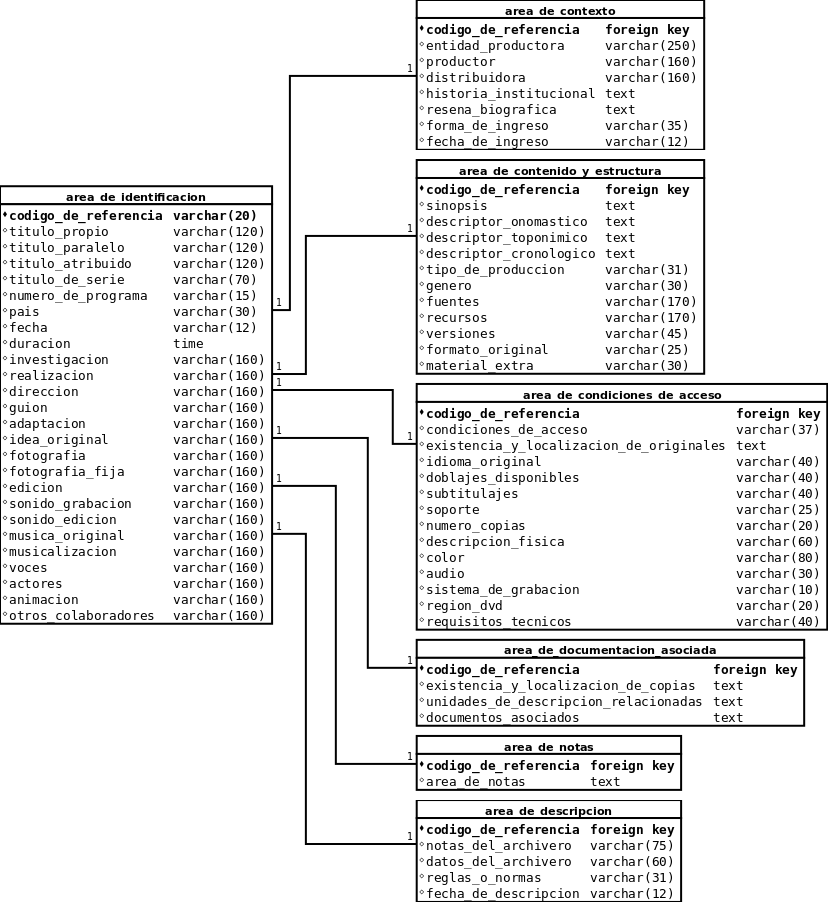
\includegraphics[keepaspectratio=true,width=\linewidth]{EntidadRelacion.png}
	%\includesvg{Diagramas/EntidadRelacion.svg}
	\caption{Diagrama Entidad-Relación que muestra el diseño de la base de datos}
	\label{fig:entidad_relacion}
\end{figure}

\subsection{Explicación del diseño de la base de datos}
Cada tabla muestra los campos que lo componen y el tipo de dato asociado, los tipos de datos que se emplean son los siguientes:
\begin{description}
	\item[varchar] \hfill \\
		Representa una cadena de caracteres (texto) de longitud variable. Se agrega entre paréntesis la longitud máxima que puede tener el texto. Este es el tipo de dato más común en la base de datos.

	\item[text] \hfill \\
		Representa una cadena de caracteres (texto) de longitud muy extensa. Es útil para descripciones como la \textit{historia institucional} o la \textit{reseña biográfica}. Aunque ofrece una longitud teóricamente ilimitada de texto, las consultas o búsquedas en este tipo de datos son más lentas que en \textbf{varchar}.
	\item[time] \hfill \\
		Representa tiempo y tiene dos utilidades: representar una hora del día (por ejemplo, las 2:15 pm) y representar un lapso de tiempo (por ejemplo, 2 horas y 15 minutos). Nos interesa el último uso para la representación de \textit{duración}.
	\item[date] \hfill \\
		Representa fechas y son especialmente útiles para campos como \textit{fecha de ingreso} o \textit{fecha de descripción}.
\end{description}

Cada tabla contiene el campo \textbf{código de referencia} porque todas las tablas hacen referencia a un archivo audiovisual que debe aparecer una sola vez en cada tabla, este tipo de relación es llamada ``1 a 1'' y es por eso que en la figura~\ref{fig:entidad_relacion} se muestran números `1' al inicio y fin de cada línea.
También el \textbf{código de referencia} es el único elemento obligatorio para todas las tablas, el resto de los campos o columnas de las tablas son opcionales (es decir, pueden quedar en blanco).

La descripción que existe en los archivos Excel repiten el campo de \textit{título propio} para cada hoja. Este detalle no se permite en la base de datos porque crearía redundancia de información (repetición de datos).

\section{Prototipos de la interfaz web}
Los prototipos o ejemplos de prueba son un diseño inicial para mostrar las características y funcionalidad principalmente de la interfaz web.

La figura~\ref{fig:prueba_conexion} muestra un ejemplo de conexión y consulta exitoso entre la página web y la base de datos. La petición resulta en obtener ciertos datos y mostrarlos en una tabla a modo de ejemplo. El detalle importante dentro del código fuente de la página web de este prototipo es que rescata valores de tres diferentes tablas con PHP y las integra en una tabla preformateada con Bootstrap.

\begin{figure}[H]
	\centering
	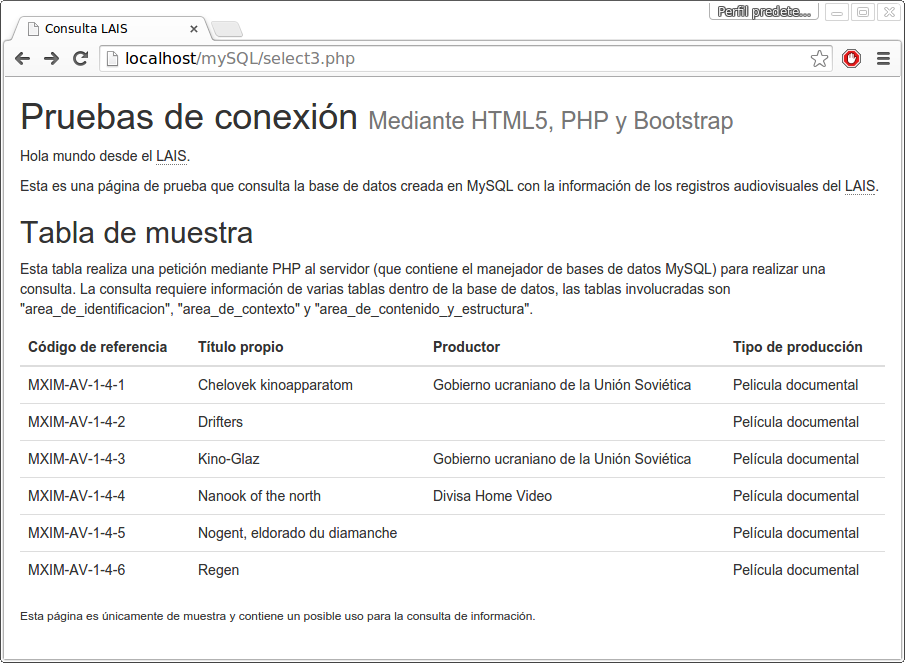
\includegraphics[keepaspectratio=true,width=\linewidth]{Prototipo_01.png}
	\caption{Prueba de conexión y consulta con la base de datos}
	\label{fig:prueba_conexion}
\end{figure}

La figura~\ref{fig:prueba_formulario} muestra un formulario básico de consulta que permite hacer búsquedas por título y filtrar la información importante que se desea ver. La figura~\ref{fig:prueba_formulario_2} muestra mas elementos de la consulta realizada en formato de lista, y muestra que es posible manipular los datos para darles el formato que queramos.

\begin{figure}[H]
	\centering
	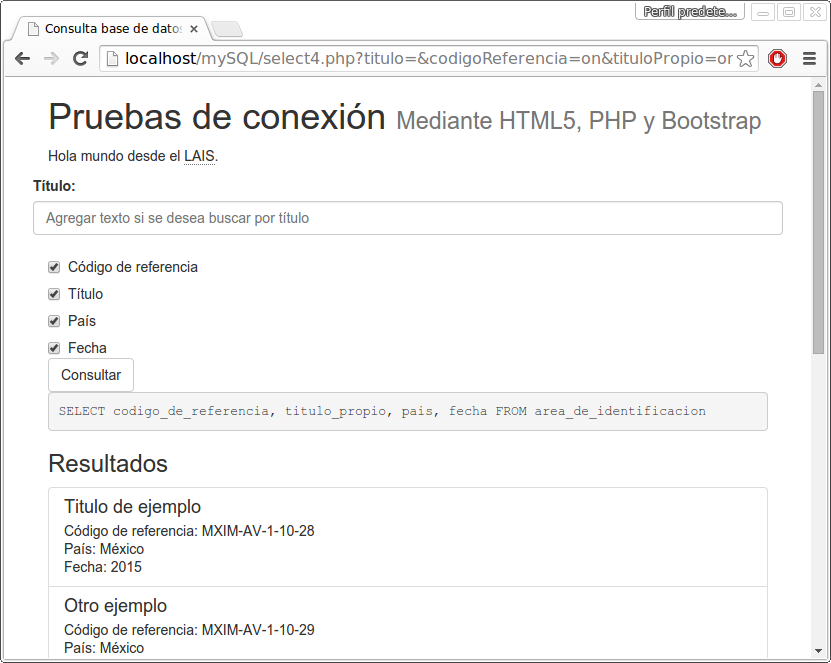
\includegraphics[keepaspectratio=true,width=\linewidth]{Prototipo_02.png}
	\caption{Prueba de búsqueda selectiva que muestra un formulario básico de consulta}
	\label{fig:prueba_formulario}
\end{figure}

\begin{figure}[H]
	\centering
	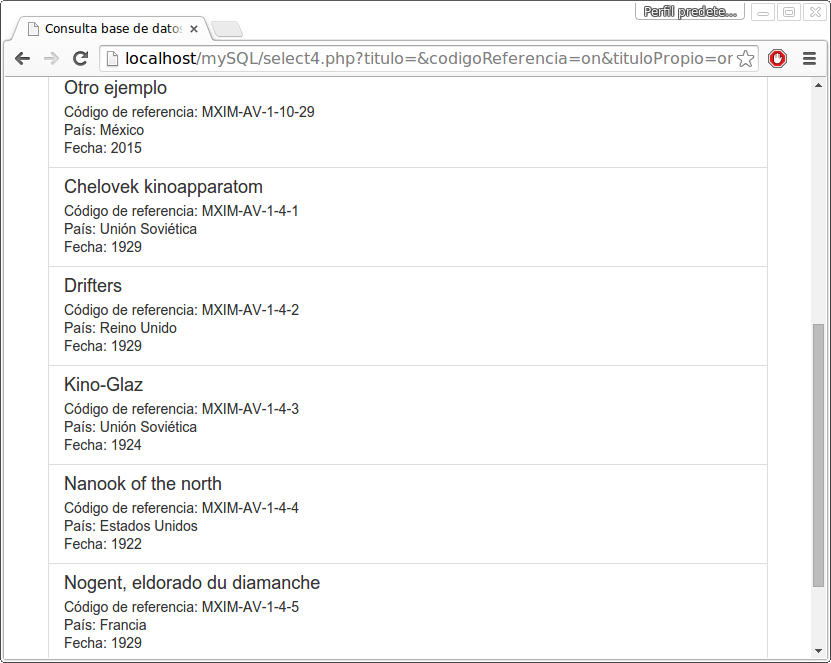
\includegraphics[keepaspectratio=true,width=\linewidth]{Prototipo_03.png}
	\caption{Algunos ejemplares en un formato de prueba para mostrar resultados de búsqueda selectiva}
	\label{fig:prueba_formulario_2}
\end{figure}

\section{Futuro desarrollo}
Se requiere de la supervisión del equipo del LAIS para aprobar el diseño de la base de datos y crear nuevos prototipos para la interfaz web que sean adecuados para las necesidades del LAIS.

En la programación se requiere crear una clase para definir un recurso audiovisual en lenguaje de programación PHP e investigar la creación dinámica de páginas que representen a cada recurso audiovisual de manera individual con toda la información posible en base a las fototecas digitales del proyecto Huellas de Luz (\url{http://lais.mora.edu.mx/huellasdeluz/}).

Se debe organizar el proyecto para subirlo a un repositorio Git para tener un manejo adecuado de versiones y el desarrollo esté organizado y sea eficiente de manejar.

\subsection{Problemas}
Listado de algunos problemas que se han encontrado durante el desarrollo y pruebas:
\begin{description}
	\item[Longitud de texto] \hfill \\
		Se debe revisar la longitud de los cadenas de texto para los campos de la base de datos (tipos de dato \textbf{varchar}). Muchos de los campos son para describir nombres de personas y tienen longitud máxima de 70 caracteres\footnote{UK Government Data Standards Catalogue \url{http://www.datadictionary.nhs.uk/data_dictionary/data_field_notes/p/pers/person_full_name_de.asp?shownav=1}}.
	\item[Fechas] \hfill \\
		El campo \textit{fecha} tiene el problema de que permite almacenar un periodo de tiempo en formato \verb|[YYYY-YYYY]|, sin embargo, para la base de datos no hay tipo especifico para determinar rangos o periodos de tiempo. \\
		Existen dos posibles soluciones: Dejar el tipo de dato para \textit{fecha} como \textit{varchar(11)} (es decir, como texto) pero las búsquedas por lapsos de tiempo serán complicadas y posiblemente inexactas. Otra alternativa es separar el campo \textit{fecha} en \textit{fecha\_inicio} y \textit{fecha\_fin}, pero requiere el preprocesamiento de la información (requiere programación) y un cambio en el diseño de la base de datos; la ventaja radica en que las búsquedas por lapsos de tiempo serán viables.
	\item[Duración] \hfill \\
		El campo \textit{duración} de la base de datos requiere que el formato sea el siguiente \verb|HH:MM:SS| o \verb|HHMMSS|. Sin embargo hay restricciones en cuanto a los número válidos para los minutos y segundos porque no pueden rebasar la cifra 60. Sin embargo, hay registros en las hojas de cálculo con valores como \verb|66:06| que signica duración de 66 minutos y 6 segundos, pero la base de datos espera que se encuentren en el formato \verb|01:06:05|. El problema se puede resolver con preprocesamiento de la información (requiere programación).
	\item[Datos nulos o cadenas vacias] \hfill \\
		En la base de datos, el valor por default es la constante \verb|NULL| y representa un elemento vacio. Sin embargo, en las hojas de cálculo el valor por default es la cadena vacia. Hay que determinar cuál será el elemento por default en el sistema.
\end{description}

\section{Notas}
La base de datos y los prototipos aun no están en línea, están en desarrollo y por el momento solo se pueden ejecutar en las máquinas del LAIS con la restricción de que el equipo de cómputo de Rodrigo (programador del LAIS) se encuentre prendido para hacer la función de servidor. Próximamente, cuando el sistema se encuentre en una etapa más avanzada de desarrollo, se subirá al servidor del LAIS.

\end{document}